% arXiv version. Build: python paper_arxiv/build.py (--bundle for the upload zip)
\documentclass[10pt]{article}
\usepackage[letterpaper,textwidth=5.5in,textheight=9in,top=1in,headheight=12pt,headsep=25pt,footskip=30pt]{geometry}
\usepackage[T1]{fontenc}
\usepackage{times,latexsym}
\usepackage{microtype}
\usepackage{url}
\usepackage{xurl}
\usepackage{natbib}
\usepackage{booktabs}
\usepackage{amsmath,amssymb}
\usepackage{graphicx}
\usepackage{xcolor}
\usepackage{adjustbox}
\usepackage{flafter}
\usepackage{needspace}
\usepackage{enumitem}
\usepackage{listings}
\usepackage{titlesec}
\usepackage[most]{tcolorbox}
\usepackage[font=small,labelfont=bf]{caption}
\definecolor{linkblue}{RGB}{0,72,150}
\usepackage[colorlinks=true,citecolor=linkblue,linkcolor=linkblue,urlcolor=linkblue]{hyperref}

\setlist{itemsep=2pt,topsep=3pt,leftmargin=*}
\lstset{basicstyle=\ttfamily\footnotesize, breaklines=true, columns=fullflexible,
  keepspaces=true, frame=single, rulecolor=\color{black!30}, upquote=true}
\setlength{\emergencystretch}{2em}

% Headings in the usual preprint style.
\titleformat{\section}{\large\bfseries}{\thesection}{0.8em}{}
\titleformat{\subsection}{\normalsize\bfseries}{\thesubsection}{0.8em}{}
\titlespacing*{\section}{0pt}{12pt plus 3pt minus 2pt}{6pt plus 2pt}
\titlespacing*{\subsection}{0pt}{9pt plus 2pt minus 2pt}{4pt plus 1pt}
\titleformat{\paragraph}[runin]{\normalsize\bfseries}{}{0pt}{}[.]
\titlespacing*{\paragraph}{0pt}{6pt plus 2pt minus 1pt}{0.6em}

% A boxed one-sentence takeaway at the end of each results section.
\newtcolorbox{takeaway}{enhanced, colback=linkblue!4, colframe=linkblue!60,
  boxrule=0.5pt, arc=2pt, left=7pt, right=7pt, top=4pt, bottom=4pt,
  fontupper=\small, before skip=8pt, after skip=8pt}

% Study 1's numbers (src/engine_b.py), the shared numbers
% (paper_tacl/make_numbers.py), then the arXiv additions
% (paper_arxiv/make_arxiv_numbers.py).

\newcommand{\Chance}{20.0\%}
\newcommand{\NFeatures}{18}
\newcommand{\EngineAAcc}{86.3\%}
\newcommand{\EngineACI}{[80.7\%, 90.5\%]}
\newcommand{\EngineAPerm}{$p < 0.001$ (0 of 1000 permutations reached the observed accuracy)}
\newcommand{\EngineAFoldMean}{85.8}
\newcommand{\EngineAFoldSD}{9.2}
\newcommand{\EngineALengthFreeRF}{63.9\%}
\newcommand{\EngineALengthFreeLR}{71.7\%}
\newcommand{\EngineAUngrouped}{85.3}
\newcommand{\LengthShareOfSignal}{33\%}
\newcommand{\LengthImportanceShare}{63.1\%}
\newcommand{\NPrompts}{38}
\newcommand{\NResponses}{190}
\newcommand{\LineupAcc}{33.7\%}
\newcommand{\LineupConcentration}{43.8\%}
\newcommand{\LineupBlameChi}{1.3}
\newcommand{\LineupBlameP}{0.857}
\newcommand{\LineupConfRho}{+0.146}
\newcommand{\LineupConfP}{5.98e-06}
\newcommand{\MechLineupRF}{29.7\%}
\newcommand{\MechLineupLR}{31.9\%}
\newcommand{\MechLineupIdentity}{38.9\%}
\newcommand{\GPTSelfLineup}{57.9\%}
\newcommand{\GPTPeerLineup}{30.3\%}
\newcommand{\GPTAdvLineup}{+27.6}
\newcommand{\GPTFALineup}{10.5\%}
\newcommand{\GPTNonSelfLineup}{39.5\%}
\newcommand{\GPTOverallLineup}{43.2\%}
\newcommand{\GPTBlameLineup}{21.5\%}
\newcommand{\ClaudeSelfLineup}{86.8\%}
\newcommand{\ClaudePeerLineup}{53.9\%}
\newcommand{\ClaudeAdvLineup}{+32.9}
\newcommand{\ClaudeFALineup}{9.2\%}
\newcommand{\ClaudeNonSelfLineup}{25.7\%}
\newcommand{\ClaudeOverallLineup}{37.9\%}
\newcommand{\ClaudeBlameLineup}{22.3\%}
\newcommand{\GeminiSelfLineup}{18.4\%}
\newcommand{\GeminiPeerLineup}{28.3\%}
\newcommand{\GeminiAdvLineup}{-9.9}
\newcommand{\GeminiFALineup}{20.4\%}
\newcommand{\GeminiNonSelfLineup}{40.8\%}
\newcommand{\GeminiOverallLineup}{36.3\%}
\newcommand{\GeminiBlameLineup}{18.8\%}
\newcommand{\GrokSelfLineup}{5.3\%}
\newcommand{\GrokPeerLineup}{28.9\%}
\newcommand{\GrokAdvLineup}{-23.7}
\newcommand{\GrokFALineup}{20.4\%}
\newcommand{\GrokNonSelfLineup}{30.9\%}
\newcommand{\GrokOverallLineup}{25.8\%}
\newcommand{\GrokBlameLineup}{17.8\%}
\newcommand{\DeepSeekSelfLineup}{21.1\%}
\newcommand{\DeepSeekPeerLineup}{21.7\%}
\newcommand{\DeepSeekAdvLineup}{-0.7}
\newcommand{\DeepSeekFALineup}{17.8\%}
\newcommand{\DeepSeekNonSelfLineup}{26.3\%}
\newcommand{\DeepSeekOverallLineup}{25.3\%}
\newcommand{\DeepSeekBlameLineup}{19.6\%}
\newcommand{\PooledNonSelfLineup}{32.6\%}
\newcommand{\SingleAcc}{30.6\%}
\newcommand{\SingleConcentration}{99.3\%}
\newcommand{\SingleBlameChi}{280.7}
\newcommand{\SingleBlameP}{1.58e-59}
\newcommand{\SingleConfRho}{+0.019}
\newcommand{\SingleConfP}{0.553}
\newcommand{\MechSingleRF}{63.0\%}
\newcommand{\MechSingleLR}{61.0\%}
\newcommand{\MechSingleIdentity}{64.9\%}
\newcommand{\GPTSelfSingle}{94.7\%}
\newcommand{\GPTPeerSingle}{61.2\%}
\newcommand{\GPTAdvSingle}{+33.6}
\newcommand{\GPTFASingle}{52.0\%}
\newcommand{\GPTNonSelfSingle}{24.3\%}
\newcommand{\GPTOverallSingle}{38.4\%}
\newcommand{\GPTBlameSingle}{45.9\%}
\newcommand{\ClaudeSelfSingle}{86.8\%}
\newcommand{\ClaudePeerSingle}{82.2\%}
\newcommand{\ClaudeAdvSingle}{+4.6}
\newcommand{\ClaudeFASingle}{8.6\%}
\newcommand{\ClaudeNonSelfSingle}{27.0\%}
\newcommand{\ClaudeOverallSingle}{38.9\%}
\newcommand{\ClaudeBlameSingle}{53.4\%}
\newcommand{\GeminiSelfSingle}{0.0\%}
\newcommand{\GeminiPeerSingle}{1.3\%}
\newcommand{\GeminiAdvSingle}{-1.3}
\newcommand{\GeminiFASingle}{0.0\%}
\newcommand{\GeminiNonSelfSingle}{32.9\%}
\newcommand{\GeminiOverallSingle}{26.3\%}
\newcommand{\GeminiBlameSingle}{0.3\%}
\newcommand{\GrokSelfSingle}{0.0\%}
\newcommand{\GrokPeerSingle}{0.7\%}
\newcommand{\GrokAdvSingle}{-0.7}
\newcommand{\GrokFASingle}{0.0\%}
\newcommand{\GrokNonSelfSingle}{33.6\%}
\newcommand{\GrokOverallSingle}{26.8\%}
\newcommand{\GrokBlameSingle}{0.1\%}
\newcommand{\DeepSeekSelfSingle}{0.0\%}
\newcommand{\DeepSeekPeerSingle}{0.7\%}
\newcommand{\DeepSeekAdvSingle}{-0.7}
\newcommand{\DeepSeekFASingle}{0.0\%}
\newcommand{\DeepSeekNonSelfSingle}{28.3\%}
\newcommand{\DeepSeekOverallSingle}{22.6\%}
\newcommand{\DeepSeekBlameSingle}{0.3\%}
\newcommand{\PooledNonSelfSingle}{29.2\%}
\newcommand{\SlotChi}{0.00}
\newcommand{\AllDistinctShare}{85.3\%}
\newcommand{\SonnetShift}{-2.5}
\newcommand{\SonnetDropped}{84.4\%}

\providecommand{\PENDING}[1]{\textcolor{red}{[#1]}}
\newcommand{\GPTAdvLineupCI}{[+10.5, +44.7]}
\newcommand{\GPTAdvLineupP}{$0.002$}
\newcommand{\GPTAdvLineupHolm}{$0.008$}
\newcommand{\GPTSelfLineupCI}{[40.8, 73.7]}
\newcommand{\GPTSelfLineupK}{22}
\newcommand{\GPTFALineupK}{16}
\newcommand{\GPTPeerLineupK}{46}
\newcommand{\GPTNonSelfLineupK}{60}
\newcommand{\GPTNonSelfLineupP}{$3.7\times10^{-8}$}
\newcommand{\GPTAdjAdvLineup}{+19.3}
\newcommand{\GPTAdjAdvLineupCI}{[+4.4, +34.2]}
\newcommand{\ClaudeAdvLineupCI}{[+21.1, +44.1]}
\newcommand{\ClaudeAdvLineupP}{$3.0\times10^{-4}$}
\newcommand{\ClaudeAdvLineupHolm}{$0.002$}
\newcommand{\ClaudeSelfLineupCI}{[71.9, 95.6]}
\newcommand{\ClaudeSelfLineupK}{33}
\newcommand{\ClaudeFALineupK}{14}
\newcommand{\ClaudePeerLineupK}{82}
\newcommand{\ClaudeNonSelfLineupK}{39}
\newcommand{\ClaudeNonSelfLineupP}{$0.085$}
\newcommand{\ClaudeAdjAdvLineup}{+35.1}
\newcommand{\ClaudeAdjAdvLineupCI}{[+21.3, +48.2]}
\newcommand{\GeminiAdvLineupCI}{[$-$23.0, +4.6]}
\newcommand{\GeminiAdvLineupP}{$0.309$}
\newcommand{\GeminiAdvLineupHolm}{$0.619$}
\newcommand{\GeminiSelfLineupCI}{[7.7, 34.3]}
\newcommand{\GeminiSelfLineupK}{7}
\newcommand{\GeminiFALineupK}{31}
\newcommand{\GeminiPeerLineupK}{43}
\newcommand{\GeminiNonSelfLineupK}{62}
\newcommand{\GeminiNonSelfLineupP}{$5.1\times10^{-9}$}
\newcommand{\GeminiAdjAdvLineup}{$-$19.3}
\newcommand{\GeminiAdjAdvLineupCI}{[$-$32.2, $-$5.9]}
\newcommand{\GrokAdvLineupCI}{[$-$32.9, $-$13.2]}
\newcommand{\GrokAdvLineupP}{$0.002$}
\newcommand{\GrokAdvLineupHolm}{$0.008$}
\newcommand{\GrokSelfLineupCI}{[0.6, 17.7]}
\newcommand{\GrokSelfLineupK}{2}
\newcommand{\GrokFALineupK}{31}
\newcommand{\GrokPeerLineupK}{44}
\newcommand{\GrokNonSelfLineupK}{47}
\newcommand{\GrokNonSelfLineupP}{$0.002$}
\newcommand{\GrokAdjAdvLineup}{$-$20.2}
\newcommand{\GrokAdjAdvLineupCI}{[$-$30.5, $-$9.6]}
\newcommand{\DeepSeekAdvLineupCI}{[$-$15.1, +15.1]}
\newcommand{\DeepSeekAdvLineupP}{$1.000$}
\newcommand{\DeepSeekAdvLineupHolm}{$1.000$}
\newcommand{\DeepSeekSelfLineupCI}{[9.6, 37.3]}
\newcommand{\DeepSeekSelfLineupK}{8}
\newcommand{\DeepSeekFALineupK}{27}
\newcommand{\DeepSeekPeerLineupK}{33}
\newcommand{\DeepSeekNonSelfLineupK}{40}
\newcommand{\DeepSeekNonSelfLineupP}{$0.054$}
\newcommand{\DeepSeekAdjAdvLineup}{+11.4}
\newcommand{\DeepSeekAdjAdvLineupCI}{[$-$7.7, +31.4]}
\newcommand{\PeerDeffLineup}{1.04}
\newcommand{\PeerNeffLineup}{146}
\newcommand{\GPTAdvSingleCI}{[+25.0, +42.1]}
\newcommand{\GPTAdvSingleP}{$4.1\times10^{-5}$}
\newcommand{\GPTAdvSingleHolm}{$2.1\times10^{-4}$}
\newcommand{\GPTSelfSingleCI}{[82.3, 99.4]}
\newcommand{\GPTSelfSingleK}{36}
\newcommand{\GPTFASingleK}{79}
\newcommand{\GPTPeerSingleK}{93}
\newcommand{\GPTNonSelfSingleK}{37}
\newcommand{\GPTNonSelfSingleP}{$0.187$}
\newcommand{\GPTAdjAdvSingle}{+29.4}
\newcommand{\GPTAdjAdvSingleCI}{[+20.2, +38.6]}
\newcommand{\ClaudeAdvSingleCI}{[$-$7.2, +14.5]}
\newcommand{\ClaudeAdvSingleP}{$0.651$}
\newcommand{\ClaudeAdvSingleHolm}{$1.000$}
\newcommand{\ClaudeSelfSingleCI}{[71.9, 95.6]}
\newcommand{\ClaudeSelfSingleK}{33}
\newcommand{\ClaudeFASingleK}{13}
\newcommand{\ClaudePeerSingleK}{125}
\newcommand{\ClaudeNonSelfSingleK}{41}
\newcommand{\ClaudeNonSelfSingleP}{$0.042$}
\newcommand{\ClaudeAdjAdvSingle}{$-$10.1}
\newcommand{\ClaudeAdjAdvSingleCI}{[$-$21.7, +0.0]}
\newcommand{\GeminiAdvSingleCI}{[$-$3.3, +0.0]}
\newcommand{\GeminiAdvSingleP}{$1.000$}
\newcommand{\GeminiAdvSingleHolm}{$1.000$}
\newcommand{\GeminiSelfSingleCI}{[0.0, 9.3]}
\newcommand{\GeminiSelfSingleK}{0}
\newcommand{\GeminiFASingleK}{0}
\newcommand{\GeminiPeerSingleK}{2}
\newcommand{\GeminiNonSelfSingleK}{50}
\newcommand{\GeminiNonSelfSingleP}{$2.2\times10^{-4}$}
\newcommand{\GeminiAdjAdvSingle}{+3.1}
\newcommand{\GeminiAdjAdvSingleCI}{[$-$0.7, +6.6]}
\newcommand{\GrokAdvSingleCI}{[$-$2.0, +0.0]}
\newcommand{\GrokAdvSingleP}{$1.000$}
\newcommand{\GrokAdvSingleHolm}{$1.000$}
\newcommand{\GrokSelfSingleCI}{[0.0, 9.3]}
\newcommand{\GrokSelfSingleK}{0}
\newcommand{\GrokFASingleK}{0}
\newcommand{\GrokPeerSingleK}{1}
\newcommand{\GrokNonSelfSingleK}{51}
\newcommand{\GrokNonSelfSingleP}{$9.6\times10^{-5}$}
\newcommand{\GrokAdjAdvSingle}{+3.1}
\newcommand{\GrokAdjAdvSingleCI}{[$-$0.7, +6.6]}
\newcommand{\DeepSeekAdvSingleCI}{[$-$2.0, +0.0]}
\newcommand{\DeepSeekAdvSingleP}{$1.000$}
\newcommand{\DeepSeekAdvSingleHolm}{$1.000$}
\newcommand{\DeepSeekSelfSingleCI}{[0.0, 9.3]}
\newcommand{\DeepSeekSelfSingleK}{0}
\newcommand{\DeepSeekFASingleK}{0}
\newcommand{\DeepSeekPeerSingleK}{1}
\newcommand{\DeepSeekNonSelfSingleK}{43}
\newcommand{\DeepSeekNonSelfSingleP}{$0.015$}
\newcommand{\DeepSeekAdjAdvSingle}{+10.1}
\newcommand{\DeepSeekAdjAdvSingleCI}{[+3.9, +15.8]}
\newcommand{\PeerDeffSingle}{0.80}
\newcommand{\PeerNeffSingle}{189}
\newcommand{\GrokSelfLineupHolm}{$0.070$}
\newcommand{\GPTMixedORLineup}{2.38}
\newcommand{\ClaudeMixedORLineup}{6.09}
\newcommand{\GeminiMixedORLineup}{0.41}
\newcommand{\GrokMixedORLineup}{0.16}
\newcommand{\DeepSeekMixedORLineup}{1.38}
\newcommand{\OWQwenLineupSelf}{56.7\%}
\newcommand{\OWQwenLineupSelfK}{68/120}
\newcommand{\OWQwenLineupPeer}{15.8\%}
\newcommand{\OWQwenLineupAdv}{+40.8}
\newcommand{\OWQwenLineupAdvCI}{[+31.1, +50.6]}
\newcommand{\OWQwenLineupP}{$<0.001$}
\newcommand{\OWQwenLineupHolm}{$<0.001$}
\newcommand{\OWQwenLineupFA}{49.2\%}
\newcommand{\OWQwenLineupFAK}{177/360}
\newcommand{\OWQwenLineupDisc}{+7.5}
\newcommand{\OWQwenLineupDiscHolm}{$0.419$}
\newcommand{\OWQwenLineupDiscLOR}{0.30}
\newcommand{\OWQwenLineupNamesSelf}{51.0\%}
\newcommand{\OWQwenLineupNonSelf}{16.4\%}
\newcommand{\OWLlamaLineupSelf}{32.5\%}
\newcommand{\OWLlamaLineupSelfK}{39/120}
\newcommand{\OWLlamaLineupPeer}{22.2\%}
\newcommand{\OWLlamaLineupAdv}{+10.3}
\newcommand{\OWLlamaLineupAdvCI}{[+1.9, +18.6]}
\newcommand{\OWLlamaLineupP}{$0.009$}
\newcommand{\OWLlamaLineupHolm}{$0.028$}
\newcommand{\OWLlamaLineupFA}{36.1\%}
\newcommand{\OWLlamaLineupFAK}{130/360}
\newcommand{\OWLlamaLineupDisc}{$-$3.6}
\newcommand{\OWLlamaLineupDiscHolm}{$1.000$}
\newcommand{\OWLlamaLineupDiscLOR}{$-$0.16}
\newcommand{\OWLlamaLineupNamesSelf}{35.2\%}
\newcommand{\OWLlamaLineupNonSelf}{16.9\%}
\newcommand{\OWMistralLineupSelf}{25.0\%}
\newcommand{\OWMistralLineupSelfK}{30/120}
\newcommand{\OWMistralLineupPeer}{20.8\%}
\newcommand{\OWMistralLineupAdv}{+4.2}
\newcommand{\OWMistralLineupAdvCI}{[$-$6.1, +14.4]}
\newcommand{\OWMistralLineupP}{$0.392$}
\newcommand{\OWMistralLineupHolm}{$0.784$}
\newcommand{\OWMistralLineupFA}{20.3\%}
\newcommand{\OWMistralLineupFAK}{73/360}
\newcommand{\OWMistralLineupDisc}{+4.7}
\newcommand{\OWMistralLineupDiscHolm}{$1.000$}
\newcommand{\OWMistralLineupDiscLOR}{0.28}
\newcommand{\OWMistralLineupNamesSelf}{21.5\%}
\newcommand{\OWMistralLineupNonSelf}{24.4\%}
\newcommand{\OWPhiLineupSelf}{20.8\%}
\newcommand{\OWPhiLineupSelfK}{25/120}
\newcommand{\OWPhiLineupPeer}{22.8\%}
\newcommand{\OWPhiLineupAdv}{$-$1.9}
\newcommand{\OWPhiLineupAdvCI}{[$-$10.6, +6.9]}
\newcommand{\OWPhiLineupP}{$0.716$}
\newcommand{\OWPhiLineupHolm}{$0.784$}
\newcommand{\OWPhiLineupFA}{22.5\%}
\newcommand{\OWPhiLineupFAK}{81/360}
\newcommand{\OWPhiLineupDisc}{$-$1.7}
\newcommand{\OWPhiLineupDiscHolm}{$1.000$}
\newcommand{\OWPhiLineupDiscLOR}{$-$0.09}
\newcommand{\OWPhiLineupNamesSelf}{22.1\%}
\newcommand{\OWPhiLineupNonSelf}{23.9\%}
\newcommand{\OWLineupAcc}{23.8\%}
\newcommand{\OWLineupBlameQwen}{28.5\%}
\newcommand{\OWLineupBlameLlama}{24.3\%}
\newcommand{\OWLineupBlameMistral}{21.7\%}
\newcommand{\OWLineupBlamePhi}{25.5\%}
\newcommand{\OWLineupTopTwo}{54.0\%}
\newcommand{\OWQwenSingleSelf}{95.0\%}
\newcommand{\OWQwenSingleSelfK}{114/120}
\newcommand{\OWQwenSinglePeer}{0.0\%}
\newcommand{\OWQwenSingleAdv}{+95.0}
\newcommand{\OWQwenSingleAdvCI}{[+90.8, +98.3]}
\newcommand{\OWQwenSingleP}{$<0.001$}
\newcommand{\OWQwenSingleHolm}{$<0.001$}
\newcommand{\OWQwenSingleFA}{93.1\%}
\newcommand{\OWQwenSingleFAK}{335/360}
\newcommand{\OWQwenSingleDisc}{+1.9}
\newcommand{\OWQwenSingleDiscHolm}{$0.884$}
\newcommand{\OWQwenSingleDiscLOR}{0.29}
\newcommand{\OWQwenSingleNamesSelf}{93.5\%}
\newcommand{\OWQwenSingleNonSelf}{2.2\%}
\newcommand{\OWLlamaSingleSelf}{100.0\%}
\newcommand{\OWLlamaSingleSelfK}{120/120}
\newcommand{\OWLlamaSinglePeer}{12.8\%}
\newcommand{\OWLlamaSingleAdv}{+87.2}
\newcommand{\OWLlamaSingleAdvCI}{[+84.2, +90.3]}
\newcommand{\OWLlamaSingleP}{$<0.001$}
\newcommand{\OWLlamaSingleHolm}{$<0.001$}
\newcommand{\OWLlamaSingleFA}{100.0\%}
\newcommand{\OWLlamaSingleFAK}{360/360}
\newcommand{\OWLlamaSingleDisc}{+0.0}
\newcommand{\OWLlamaSingleDiscHolm}{$1.000$}
\newcommand{\OWLlamaSingleDiscLOR}{$-$1.10}
\newcommand{\OWLlamaSingleNamesSelf}{100.0\%}
\newcommand{\OWLlamaSingleNonSelf}{0.0\%}
\newcommand{\OWMistralSingleSelf}{10.0\%}
\newcommand{\OWMistralSingleSelfK}{12/120}
\newcommand{\OWMistralSinglePeer}{22.2\%}
\newcommand{\OWMistralSingleAdv}{$-$12.2}
\newcommand{\OWMistralSingleAdvCI}{[$-$18.1, $-$5.8]}
\newcommand{\OWMistralSingleP}{$0.009$}
\newcommand{\OWMistralSingleHolm}{$0.019$}
\newcommand{\OWMistralSingleFA}{6.1\%}
\newcommand{\OWMistralSingleFAK}{22/360}
\newcommand{\OWMistralSingleDisc}{+3.9}
\newcommand{\OWMistralSingleDiscHolm}{$0.503$}
\newcommand{\OWMistralSingleDiscLOR}{0.55}
\newcommand{\OWMistralSingleNamesSelf}{7.1\%}
\newcommand{\OWMistralSingleNonSelf}{33.3\%}
\newcommand{\OWPhiSingleSelf}{35.8\%}
\newcommand{\OWPhiSingleSelfK}{43/120}
\newcommand{\OWPhiSinglePeer}{23.1\%}
\newcommand{\OWPhiSingleAdv}{+12.8}
\newcommand{\OWPhiSingleAdvCI}{[+2.5, +22.8]}
\newcommand{\OWPhiSingleP}{$0.014$}
\newcommand{\OWPhiSingleHolm}{$0.019$}
\newcommand{\OWPhiSingleFA}{29.7\%}
\newcommand{\OWPhiSingleFAK}{107/360}
\newcommand{\OWPhiSingleDisc}{+6.1}
\newcommand{\OWPhiSingleDiscHolm}{$0.340$}
\newcommand{\OWPhiSingleDiscLOR}{0.28}
\newcommand{\OWPhiSingleNamesSelf}{31.2\%}
\newcommand{\OWPhiSingleNonSelf}{22.5\%}
\newcommand{\OWSingleAcc}{25.9\%}
\newcommand{\OWSingleBlameQwen}{23.8\%}
\newcommand{\OWSingleBlameLlama}{34.1\%}
\newcommand{\OWSingleBlameMistral}{18.8\%}
\newcommand{\OWSingleBlamePhi}{23.4\%}
\newcommand{\OWSingleTopTwo}{57.9\%}
\newcommand{\OWQwenBinaryAUC}{0.45}
\newcommand{\OWQwenBinaryAUCCI}{[0.41, 0.49]}
\newcommand{\OWQwenBinaryAUCHolm}{$0.135$}
\newcommand{\OWQwenBinaryHit}{51.7\%}
\newcommand{\OWQwenBinaryFA}{58.6\%}
\newcommand{\OWLlamaBinaryAUC}{0.53}
\newcommand{\OWLlamaBinaryAUCCI}{[0.48, 0.58]}
\newcommand{\OWLlamaBinaryAUCHolm}{$0.348$}
\newcommand{\OWLlamaBinaryHit}{85.8\%}
\newcommand{\OWLlamaBinaryFA}{85.6\%}
\newcommand{\OWMistralBinaryAUC}{0.41}
\newcommand{\OWMistralBinaryAUCCI}{[0.36, 0.46]}
\newcommand{\OWMistralBinaryAUCHolm}{$0.002$}
\newcommand{\OWMistralBinaryHit}{99.2\%}
\newcommand{\OWMistralBinaryFA}{99.4\%}
\newcommand{\OWPhiBinaryAUC}{0.53}
\newcommand{\OWPhiBinaryAUCCI}{[0.49, 0.57]}
\newcommand{\OWPhiBinaryAUCHolm}{$0.348$}
\newcommand{\OWPhiBinaryHit}{4.2\%}
\newcommand{\OWPhiBinaryFA}{1.4\%}
\newcommand{\OWQwenBinaryCodeAUC}{0.48}
\newcommand{\OWLlamaBinaryCodeAUC}{0.64}
\newcommand{\OWMistralBinaryCodeAUC}{0.52}
\newcommand{\OWPhiBinaryCodeAUC}{0.50}
\newcommand{\OWQwenBinaryMathAUC}{0.53}
\newcommand{\OWLlamaBinaryMathAUC}{0.50}
\newcommand{\OWMistralBinaryMathAUC}{0.42}
\newcommand{\OWPhiBinaryMathAUC}{0.58}
\newcommand{\OWQwenBinaryProseAUC}{0.47}
\newcommand{\OWLlamaBinaryProseAUC}{0.51}
\newcommand{\OWMistralBinaryProseAUC}{0.37}
\newcommand{\OWPhiBinaryProseAUC}{0.56}
\newcommand{\OWQwenBinaryShortAUC}{0.29}
\newcommand{\OWLlamaBinaryShortAUC}{0.51}
\newcommand{\OWMistralBinaryShortAUC}{0.40}
\newcommand{\OWPhiBinaryShortAUC}{0.41}
\newcommand{\OWBinaryAUCGenreMax}{0.64}
\newcommand{\OWBinaryAUCGenreMaxCI}{[0.50, 0.79]}
\newcommand{\OWBinaryAUCGenreMaxWho}{Llama, code}
\newcommand{\OWQwenBinaryAUCGenreLo}{0.29}
\newcommand{\OWQwenBinaryAUCGenreHi}{0.53}
\newcommand{\OWLlamaBinaryAUCGenreLo}{0.50}
\newcommand{\OWLlamaBinaryAUCGenreHi}{0.64}
\newcommand{\OWMistralBinaryAUCGenreLo}{0.37}
\newcommand{\OWMistralBinaryAUCGenreHi}{0.52}
\newcommand{\OWPhiBinaryAUCGenreLo}{0.41}
\newcommand{\OWPhiBinaryAUCGenreHi}{0.58}
\newcommand{\OWQwenOnPolAUC}{0.88}
\newcommand{\OWQwenOnPolAUCCI}{[0.85, 0.91]}
\newcommand{\OWQwenOnPolAUCHolm}{$<0.001$}
\newcommand{\OWQwenOnPolHit}{81.7\%}
\newcommand{\OWQwenOnPolFA}{22.8\%}
\newcommand{\OWLlamaOnPolAUC}{0.57}
\newcommand{\OWLlamaOnPolAUCCI}{[0.50, 0.63]}
\newcommand{\OWLlamaOnPolAUCHolm}{$0.002$}
\newcommand{\OWLlamaOnPolHit}{14.2\%}
\newcommand{\OWLlamaOnPolFA}{6.4\%}
\newcommand{\OWMistralOnPolAUC}{0.89}
\newcommand{\OWMistralOnPolAUCCI}{[0.86, 0.92]}
\newcommand{\OWMistralOnPolAUCHolm}{$<0.001$}
\newcommand{\OWMistralOnPolHit}{100.0\%}
\newcommand{\OWMistralOnPolFA}{98.6\%}
\newcommand{\OWPhiOnPolAUC}{0.66}
\newcommand{\OWPhiOnPolAUCCI}{[0.63, 0.68]}
\newcommand{\OWPhiOnPolAUCHolm}{$<0.001$}
\newcommand{\OWPhiOnPolHit}{35.8\%}
\newcommand{\OWPhiOnPolFA}{17.5\%}
\newcommand{\OWQwenOnPolCodeAUC}{0.99}
\newcommand{\OWLlamaOnPolCodeAUC}{1.00}
\newcommand{\OWMistralOnPolCodeAUC}{0.99}
\newcommand{\OWPhiOnPolCodeAUC}{0.89}
\newcommand{\OWQwenOnPolMathAUC}{0.79}
\newcommand{\OWLlamaOnPolMathAUC}{0.33}
\newcommand{\OWMistralOnPolMathAUC}{0.82}
\newcommand{\OWPhiOnPolMathAUC}{0.55}
\newcommand{\OWQwenOnPolProseAUC}{0.86}
\newcommand{\OWLlamaOnPolProseAUC}{0.30}
\newcommand{\OWMistralOnPolProseAUC}{0.89}
\newcommand{\OWPhiOnPolProseAUC}{0.76}
\newcommand{\OWQwenOnPolShortAUC}{0.98}
\newcommand{\OWLlamaOnPolShortAUC}{0.93}
\newcommand{\OWMistralOnPolShortAUC}{0.98}
\newcommand{\OWPhiOnPolShortAUC}{0.84}
\newcommand{\OWOnPolAUCGenreMax}{1.00}
\newcommand{\OWOnPolAUCGenreMaxCI}{[0.98, 1.00]}
\newcommand{\OWOnPolAUCGenreMaxWho}{Llama, code}
\newcommand{\OWQwenOnPolAUCGenreLo}{0.79}
\newcommand{\OWQwenOnPolAUCGenreHi}{0.99}
\newcommand{\OWLlamaOnPolAUCGenreLo}{0.30}
\newcommand{\OWLlamaOnPolAUCGenreHi}{1.00}
\newcommand{\OWMistralOnPolAUCGenreLo}{0.82}
\newcommand{\OWMistralOnPolAUCGenreHi}{0.99}
\newcommand{\OWPhiOnPolAUCGenreLo}{0.55}
\newcommand{\OWPhiOnPolAUCGenreHi}{0.89}
\newcommand{\OWQwenOnPolResAUC}{0.70}
\newcommand{\OWQwenOnPolResAUCCI}{[0.65, 0.74]}
\newcommand{\OWQwenOnPolResAUCHolm}{$<0.001$}
\newcommand{\OWQwenOnPolResHit}{50.0\%}
\newcommand{\OWQwenOnPolResFA}{24.2\%}
\newcommand{\OWLlamaOnPolResAUC}{0.42}
\newcommand{\OWLlamaOnPolResAUCCI}{[0.37, 0.46]}
\newcommand{\OWLlamaOnPolResAUCHolm}{$<0.001$}
\newcommand{\OWLlamaOnPolResHit}{1.7\%}
\newcommand{\OWLlamaOnPolResFA}{8.9\%}
\newcommand{\OWMistralOnPolResAUC}{0.43}
\newcommand{\OWMistralOnPolResAUCCI}{[0.39, 0.48]}
\newcommand{\OWMistralOnPolResAUCHolm}{$0.002$}
\newcommand{\OWMistralOnPolResHit}{96.7\%}
\newcommand{\OWMistralOnPolResFA}{98.9\%}
\newcommand{\OWPhiOnPolResAUC}{0.58}
\newcommand{\OWPhiOnPolResAUCCI}{[0.55, 0.61]}
\newcommand{\OWPhiOnPolResAUCHolm}{$<0.001$}
\newcommand{\OWPhiOnPolResHit}{20.0\%}
\newcommand{\OWPhiOnPolResFA}{18.1\%}
\newcommand{\OWQwenOnPolResCodeAUC}{0.76}
\newcommand{\OWLlamaOnPolResCodeAUC}{0.71}
\newcommand{\OWMistralOnPolResCodeAUC}{0.52}
\newcommand{\OWPhiOnPolResCodeAUC}{0.65}
\newcommand{\OWQwenOnPolResMathAUC}{0.70}
\newcommand{\OWLlamaOnPolResMathAUC}{0.37}
\newcommand{\OWMistralOnPolResMathAUC}{0.34}
\newcommand{\OWPhiOnPolResMathAUC}{0.61}
\newcommand{\OWQwenOnPolResProseAUC}{0.60}
\newcommand{\OWLlamaOnPolResProseAUC}{0.28}
\newcommand{\OWMistralOnPolResProseAUC}{0.45}
\newcommand{\OWPhiOnPolResProseAUC}{0.69}
\newcommand{\OWQwenOnPolResShortAUC}{0.82}
\newcommand{\OWLlamaOnPolResShortAUC}{0.43}
\newcommand{\OWMistralOnPolResShortAUC}{0.36}
\newcommand{\OWPhiOnPolResShortAUC}{0.50}
\newcommand{\OWOnPolResAUCGenreMax}{0.82}
\newcommand{\OWOnPolResAUCGenreMaxCI}{[0.75, 0.90]}
\newcommand{\OWOnPolResAUCGenreMaxWho}{Qwen, short}
\newcommand{\OWQwenOnPolResAUCGenreLo}{0.60}
\newcommand{\OWQwenOnPolResAUCGenreHi}{0.82}
\newcommand{\OWLlamaOnPolResAUCGenreLo}{0.28}
\newcommand{\OWLlamaOnPolResAUCGenreHi}{0.71}
\newcommand{\OWMistralOnPolResAUCGenreLo}{0.34}
\newcommand{\OWMistralOnPolResAUCGenreHi}{0.52}
\newcommand{\OWPhiOnPolResAUCGenreLo}{0.50}
\newcommand{\OWPhiOnPolResAUCGenreHi}{0.69}
\newcommand{\OWQwenLikAcc}{100.0\%}
\newcommand{\OWQwenLikRawAcc}{100.0\%}
\newcommand{\OWQwenLikAUC}{1.00}
\newcommand{\OWLlamaLikAcc}{100.0\%}
\newcommand{\OWLlamaLikRawAcc}{98.3\%}
\newcommand{\OWLlamaLikAUC}{1.00}
\newcommand{\OWMistralLikAcc}{100.0\%}
\newcommand{\OWMistralLikRawAcc}{100.0\%}
\newcommand{\OWMistralLikAUC}{1.00}
\newcommand{\OWPhiLikAcc}{100.0\%}
\newcommand{\OWPhiLikRawAcc}{97.5\%}
\newcommand{\OWPhiLikAUC}{1.00}
\newcommand{\OWLikCondAccMin}{100.0\%}
\newcommand{\OWLikCondAccMax}{100.0\%}
\newcommand{\OWLikCondAUCMin}{1.00}
\newcommand{\OWLikCondRawMin}{97.5\%}
\newcommand{\OWLikCondRawMax}{100.0\%}
\newcommand{\OWLikUncAccMin}{90.8\%}
\newcommand{\OWLikUncAccMax}{100.0\%}
\newcommand{\OWLikUncAUCMin}{0.95}
\newcommand{\OWLikUncRawMin}{58.3\%}
\newcommand{\OWLikUncRawMax}{86.7\%}
\newcommand{\OWFamTests}{10}
\newcommand{\OWFamMinP}{$0.006$}
\newcommand{\OWFamMinHolm}{$0.065$}
\newcommand{\OWFamMinWho}{Qwen, single text}
\newcommand{\OWFamUntestable}{2}
\newcommand{\OWQwenFamLineup}{+0.11}
\newcommand{\OWQwenFamLineupP}{$0.187$}
\newcommand{\OWLlamaFamLineup}{+0.03}
\newcommand{\OWLlamaFamLineupP}{$0.765$}
\newcommand{\OWMistralFamLineup}{$-$0.05}
\newcommand{\OWMistralFamLineupP}{$0.675$}
\newcommand{\OWPhiFamLineup}{$-$0.16}
\newcommand{\OWPhiFamLineupP}{$0.247$}
\newcommand{\OWQwenFamSingle}{$-$0.71}
\newcommand{\OWQwenFamSingleP}{$0.006$}
\newcommand{\OWMistralFamSingle}{$-$0.32}
\newcommand{\OWMistralFamSingleP}{$0.178$}
\newcommand{\OWPhiFamSingle}{+0.77}
\newcommand{\OWPhiFamSingleP}{$0.571$}
\newcommand{\OWQwenFamBinary}{+0.15}
\newcommand{\OWQwenFamBinaryP}{$0.244$}
\newcommand{\OWLlamaFamBinary}{+0.02}
\newcommand{\OWLlamaFamBinaryP}{$0.959$}
\newcommand{\OWPhiFamBinary}{+1.05}
\newcommand{\OWPhiFamBinaryP}{$0.551$}
\newcommand{\OWQwenQualSelfPref}{+0.04}
\newcommand{\OWQwenQualSelfPrefCI}{[$-$0.02, +0.10]}
\newcommand{\OWLlamaQualSelfPref}{+0.01}
\newcommand{\OWLlamaQualSelfPrefCI}{[$-$0.04, +0.06]}
\newcommand{\OWMistralQualSelfPref}{+0.11}
\newcommand{\OWMistralQualSelfPrefCI}{[$-$0.00, +0.22]}
\newcommand{\OWPhiQualSelfPref}{+0.02}
\newcommand{\OWPhiQualSelfPrefCI}{[$-$0.04, +0.08]}
\newcommand{\OWQualSelfPrefMin}{+0.01}
\newcommand{\OWQualSelfPrefMax}{+0.11}
\newcommand{\OWNJudgments}{1{,}920}
\newcommand{\OWNResponses}{480}
\newcommand{\OWNPrompts}{120}
\newcommand{\RationaleValidation}{Two LLM annotators labelled a stratified sample of 150 reasons from the codebook alone; the rules agree with the blind one at 97\% precision and 96\% recall (Appendix~\ref{app:rationales}).}
\newcommand{\RationaleHumanAppendix}{}
\newcommand{\FXLineupAcc}{29.7\%}
\newcommand{\FXLineupTopTwo}{42.4\%}
\newcommand{\FXGPTLineupSelf}{19.2\%}
\newcommand{\FXGPTLineupPeer}{15.0\%}
\newcommand{\FXGPTLineupFA}{20.4\%}
\newcommand{\FXGPTLineupAdv}{+4.2}
\newcommand{\FXGPTLineupAdvCI}{[$-$3.3, +12.1]}
\newcommand{\FXGPTLineupHolm}{$1.000$}
\newcommand{\FXGPTLineupDisc}{$-$1.2}
\newcommand{\FXGPTLineupDiscHolm}{$0.846$}
\newcommand{\FXGPTLineupNamesSelf}{20.2\%}
\newcommand{\FXClaudeLineupSelf}{56.7\%}
\newcommand{\FXClaudeLineupPeer}{50.4\%}
\newcommand{\FXClaudeLineupFA}{12.7\%}
\newcommand{\FXClaudeLineupAdv}{+6.2}
\newcommand{\FXClaudeLineupAdvCI}{[$-$2.5, +14.8]}
\newcommand{\FXClaudeLineupHolm}{$1.000$}
\newcommand{\FXClaudeLineupDisc}{+44.0}
\newcommand{\FXClaudeLineupDiscHolm}{$<0.001$}
\newcommand{\FXClaudeLineupNamesSelf}{21.5\%}
\newcommand{\FXGeminiLineupSelf}{26.7\%}
\newcommand{\FXGeminiLineupPeer}{31.9\%}
\newcommand{\FXGeminiLineupFA}{18.3\%}
\newcommand{\FXGeminiLineupAdv}{$-$5.2}
\newcommand{\FXGeminiLineupAdvCI}{[$-$14.4, +3.8]}
\newcommand{\FXGeminiLineupHolm}{$1.000$}
\newcommand{\FXGeminiLineupDisc}{+8.3}
\newcommand{\FXGeminiLineupDiscHolm}{$0.245$}
\newcommand{\FXGeminiLineupNamesSelf}{20.0\%}
\newcommand{\FXGrokLineupSelf}{32.5\%}
\newcommand{\FXGrokLineupPeer}{30.2\%}
\newcommand{\FXGrokLineupFA}{16.2\%}
\newcommand{\FXGrokLineupAdv}{+2.3}
\newcommand{\FXGrokLineupAdvCI}{[$-$7.1, +11.9]}
\newcommand{\FXGrokLineupHolm}{$1.000$}
\newcommand{\FXGrokLineupDisc}{+16.2}
\newcommand{\FXGrokLineupDiscHolm}{$0.003$}
\newcommand{\FXGrokLineupNamesSelf}{19.5\%}
\newcommand{\FXDeepSeekLineupSelf}{21.7\%}
\newcommand{\FXDeepSeekLineupPeer}{18.8\%}
\newcommand{\FXDeepSeekLineupFA}{17.7\%}
\newcommand{\FXDeepSeekLineupAdv}{+2.9}
\newcommand{\FXDeepSeekLineupAdvCI}{[$-$5.2, +11.5]}
\newcommand{\FXDeepSeekLineupHolm}{$1.000$}
\newcommand{\FXDeepSeekLineupDisc}{+4.0}
\newcommand{\FXDeepSeekLineupDiscHolm}{$0.846$}
\newcommand{\FXDeepSeekLineupNamesSelf}{18.5\%}
\newcommand{\FXGPTLineupCodeAdv}{$-$10.0}
\newcommand{\FXGPTLineupCodeDisc}{$-$12.5}
\newcommand{\FXClaudeLineupCodeAdv}{+0.0}
\newcommand{\FXClaudeLineupCodeDisc}{+30.0}
\newcommand{\FXGeminiLineupCodeAdv}{$-$2.5}
\newcommand{\FXGeminiLineupCodeDisc}{+18.7}
\newcommand{\FXGrokLineupCodeAdv}{+8.8}
\newcommand{\FXGrokLineupCodeDisc}{+50.0}
\newcommand{\FXDeepSeekLineupCodeAdv}{+6.2}
\newcommand{\FXDeepSeekLineupCodeDisc}{+12.5}
\newcommand{\FXGPTLineupMathAdv}{+10.0}
\newcommand{\FXGPTLineupMathDisc}{+0.0}
\newcommand{\FXClaudeLineupMathAdv}{$-$1.3}
\newcommand{\FXClaudeLineupMathDisc}{$-$6.2}
\newcommand{\FXGeminiLineupMathAdv}{$-$10.0}
\newcommand{\FXGeminiLineupMathDisc}{$-$6.2}
\newcommand{\FXGrokLineupMathAdv}{+5.0}
\newcommand{\FXGrokLineupMathDisc}{+18.7}
\newcommand{\FXDeepSeekLineupMathAdv}{+15.0}
\newcommand{\FXDeepSeekLineupMathDisc}{+13.7}
\newcommand{\FXGPTLineupProseAdv}{+8.3}
\newcommand{\FXGPTLineupProseDisc}{+6.2}
\newcommand{\FXClaudeLineupProseAdv}{+12.5}
\newcommand{\FXClaudeLineupProseDisc}{+69.6}
\newcommand{\FXGeminiLineupProseAdv}{$-$5.8}
\newcommand{\FXGeminiLineupProseDisc}{+10.4}
\newcommand{\FXGrokLineupProseAdv}{$-$2.9}
\newcommand{\FXGrokLineupProseDisc}{+5.4}
\newcommand{\FXDeepSeekLineupProseAdv}{+2.1}
\newcommand{\FXDeepSeekLineupProseDisc}{+3.3}
\newcommand{\FXGPTLineupShortAdv}{+0.0}
\newcommand{\FXGPTLineupShortDisc}{$-$13.7}
\newcommand{\FXClaudeLineupShortAdv}{+1.3}
\newcommand{\FXClaudeLineupShortDisc}{+31.2}
\newcommand{\FXGeminiLineupShortAdv}{$-$1.3}
\newcommand{\FXGeminiLineupShortDisc}{+6.2}
\newcommand{\FXGrokLineupShortAdv}{+8.8}
\newcommand{\FXGrokLineupShortDisc}{+12.5}
\newcommand{\FXDeepSeekLineupShortAdv}{$-$10.0}
\newcommand{\FXDeepSeekLineupShortDisc}{$-$12.5}
\newcommand{\FXSingleAcc}{25.8\%}
\newcommand{\FXSingleTopTwo}{95.7\%}
\newcommand{\FXGPTSingleSelf}{83.3\%}
\newcommand{\FXGPTSinglePeer}{63.1\%}
\newcommand{\FXGPTSingleFA}{84.4\%}
\newcommand{\FXGPTSingleAdv}{+20.2}
\newcommand{\FXGPTSingleAdvCI}{[+13.5, +26.7]}
\newcommand{\FXGPTSingleHolm}{$<0.001$}
\newcommand{\FXGPTSingleDisc}{$-$1.0}
\newcommand{\FXGPTSingleDiscHolm}{$1.000$}
\newcommand{\FXGPTSingleNamesSelf}{84.2\%}
\newcommand{\FXClaudeSingleSelf}{40.8\%}
\newcommand{\FXClaudeSinglePeer}{49.8\%}
\newcommand{\FXClaudeSingleFA}{3.1\%}
\newcommand{\FXClaudeSingleAdv}{$-$9.0}
\newcommand{\FXClaudeSingleAdvCI}{[$-$16.0, $-$1.5]}
\newcommand{\FXClaudeSingleHolm}{$0.115$}
\newcommand{\FXClaudeSingleDisc}{+37.7}
\newcommand{\FXClaudeSingleDiscHolm}{$<0.001$}
\newcommand{\FXClaudeSingleNamesSelf}{10.7\%}
\newcommand{\FXGeminiSingleSelf}{8.3\%}
\newcommand{\FXGeminiSinglePeer}{4.0\%}
\newcommand{\FXGeminiSingleFA}{4.8\%}
\newcommand{\FXGeminiSingleAdv}{+4.4}
\newcommand{\FXGeminiSingleAdvCI}{[$-$0.4, +9.6]}
\newcommand{\FXGeminiSingleHolm}{$0.115$}
\newcommand{\FXGeminiSingleDisc}{+3.5}
\newcommand{\FXGeminiSingleDiscHolm}{$0.602$}
\newcommand{\FXGeminiSingleNamesSelf}{5.5\%}
\newcommand{\FXGrokSingleSelf}{1.7\%}
\newcommand{\FXGrokSinglePeer}{0.0\%}
\newcommand{\FXGrokSingleFA}{0.6\%}
\newcommand{\FXGrokSingleAdv}{+1.7}
\newcommand{\FXGrokSingleAdvCI}{[+0.0, +4.2]}
\newcommand{\FXGrokSingleHolm}{$0.115$}
\newcommand{\FXGrokSingleDisc}{+1.0}
\newcommand{\FXGrokSingleDiscHolm}{$1.000$}
\newcommand{\FXGrokSingleNamesSelf}{0.8\%}
\newcommand{\FXDeepSeekSingleSelf}{0.0\%}
\newcommand{\FXDeepSeekSinglePeer}{10.6\%}
\newcommand{\FXDeepSeekSingleFA}{0.0\%}
\newcommand{\FXDeepSeekSingleAdv}{$-$10.6}
\newcommand{\FXDeepSeekSingleAdvCI}{[$-$12.9, $-$8.3]}
\newcommand{\FXDeepSeekSingleHolm}{$0.001$}
\newcommand{\FXDeepSeekSingleDisc}{+0.0}
\newcommand{\FXDeepSeekSingleDiscHolm}{$1.000$}
\newcommand{\FXDeepSeekSingleNamesSelf}{0.0\%}
\newcommand{\FXGPTSingleCodeAdv}{+40.0}
\newcommand{\FXGPTSingleCodeDisc}{$-$8.8}
\newcommand{\FXClaudeSingleCodeAdv}{$-$48.8}
\newcommand{\FXClaudeSingleCodeDisc}{$-$3.8}
\newcommand{\FXGeminiSingleCodeAdv}{+27.5}
\newcommand{\FXGeminiSingleCodeDisc}{+27.5}
\newcommand{\FXGrokSingleCodeAdv}{+10.0}
\newcommand{\FXGrokSingleCodeDisc}{+10.0}
\newcommand{\FXDeepSeekSingleCodeAdv}{$-$3.8}
\newcommand{\FXDeepSeekSingleCodeDisc}{+0.0}
\newcommand{\FXGPTSingleMathAdv}{+11.3}
\newcommand{\FXGPTSingleMathDisc}{+3.7}
\newcommand{\FXClaudeSingleMathAdv}{+7.5}
\newcommand{\FXClaudeSingleMathDisc}{+15.0}
\newcommand{\FXGeminiSingleMathAdv}{+11.3}
\newcommand{\FXGeminiSingleMathDisc}{$-$1.2}
\newcommand{\FXGrokSingleMathAdv}{+0.0}
\newcommand{\FXGrokSingleMathDisc}{$-$1.2}
\newcommand{\FXDeepSeekSingleMathAdv}{$-$17.5}
\newcommand{\FXDeepSeekSingleMathDisc}{+0.0}
\newcommand{\FXGPTSingleProseAdv}{+21.2}
\newcommand{\FXGPTSingleProseDisc}{$-$0.4}
\newcommand{\FXClaudeSingleProseAdv}{$-$2.1}
\newcommand{\FXClaudeSingleProseDisc}{+70.4}
\newcommand{\FXGeminiSingleProseAdv}{$-$3.3}
\newcommand{\FXGeminiSingleProseDisc}{$-$0.8}
\newcommand{\FXGrokSingleProseAdv}{+0.0}
\newcommand{\FXGrokSingleProseDisc}{$-$0.4}
\newcommand{\FXDeepSeekSingleProseAdv}{$-$14.2}
\newcommand{\FXDeepSeekSingleProseDisc}{+0.0}
\newcommand{\FXGPTSingleShortAdv}{+6.2}
\newcommand{\FXGPTSingleShortDisc}{+0.0}
\newcommand{\FXClaudeSingleShortAdv}{$-$6.2}
\newcommand{\FXClaudeSingleShortDisc}{+3.8}
\newcommand{\FXGeminiSingleShortAdv}{$-$2.5}
\newcommand{\FXGeminiSingleShortDisc}{$-$2.5}
\newcommand{\FXGrokSingleShortAdv}{+0.0}
\newcommand{\FXGrokSingleShortDisc}{$-$1.2}
\newcommand{\FXDeepSeekSingleShortAdv}{+0.0}
\newcommand{\FXDeepSeekSingleShortDisc}{+0.0}
\newcommand{\FXSingleSentence}{One text at a time (3,000 judgments), the judges again send \FXSingleTopTwo{} of their guesses to GPT or Claude. GPT names itself on \FXGPTSingleNamesSelf{} of all texts, whoever wrote them, which earns it a significant self-advantage (\FXGPTSingleAdv{}, Holm $p$~\FXGPTSingleHolm{}) with no discrimination at all (\FXGPTSingleDisc{}); Claude names itself on few texts but mostly on its own (hit minus false-alarm rate \FXClaudeSingleDisc{}).}
\newcommand{\FXOldLineupAcc}{31.9\%}
\newcommand{\FXOldGPTLineupSelf}{28.9\%}
\newcommand{\FXOldGPTLineupPeer}{16.4\%}
\newcommand{\FXOldGPTLineupFA}{17.8\%}
\newcommand{\FXOldGPTLineupAdv}{+12.5}
\newcommand{\FXOldGPTLineupHolm}{$0.404$}
\newcommand{\FXOldGPTLineupDisc}{+11.2}
\newcommand{\FXOldGPTLineupDiscHolm}{$0.649$}
\newcommand{\FXOldClaudeLineupSelf}{81.6\%}
\newcommand{\FXOldClaudeLineupPeer}{63.8\%}
\newcommand{\FXOldClaudeLineupFA}{7.9\%}
\newcommand{\FXOldClaudeLineupAdv}{+17.8}
\newcommand{\FXOldClaudeLineupHolm}{$0.283$}
\newcommand{\FXOldClaudeLineupDisc}{+73.7}
\newcommand{\FXOldClaudeLineupDiscHolm}{$<0.001$}
\newcommand{\FXOldGeminiLineupSelf}{34.2\%}
\newcommand{\FXOldGeminiLineupPeer}{30.9\%}
\newcommand{\FXOldGeminiLineupFA}{16.4\%}
\newcommand{\FXOldGeminiLineupAdv}{+3.3}
\newcommand{\FXOldGeminiLineupHolm}{$1.000$}
\newcommand{\FXOldGeminiLineupDisc}{+17.8}
\newcommand{\FXOldGeminiLineupDiscHolm}{$0.145$}
\newcommand{\FXOldGrokLineupSelf}{21.1\%}
\newcommand{\FXOldGrokLineupPeer}{25.0\%}
\newcommand{\FXOldGrokLineupFA}{17.8\%}
\newcommand{\FXOldGrokLineupAdv}{$-$3.9}
\newcommand{\FXOldGrokLineupHolm}{$1.000$}
\newcommand{\FXOldGrokLineupDisc}{+3.3}
\newcommand{\FXOldGrokLineupDiscHolm}{$1.000$}
\newcommand{\FXOldDeepSeekLineupSelf}{15.8\%}
\newcommand{\FXOldDeepSeekLineupPeer}{17.8\%}
\newcommand{\FXOldDeepSeekLineupFA}{17.8\%}
\newcommand{\FXOldDeepSeekLineupAdv}{$-$2.0}
\newcommand{\FXOldDeepSeekLineupHolm}{$1.000$}
\newcommand{\FXOldDeepSeekLineupDisc}{$-$2.0}
\newcommand{\FXOldDeepSeekLineupDiscHolm}{$1.000$}
\newcommand{\FXOldLineupMaxAbsAdv}{18}
\newcommand{\FXNewLineupAcc}{28.6\%}
\newcommand{\FXNewGPTLineupSelf}{14.6\%}
\newcommand{\FXNewGPTLineupPeer}{14.3\%}
\newcommand{\FXNewGPTLineupFA}{21.6\%}
\newcommand{\FXNewGPTLineupAdv}{+0.3}
\newcommand{\FXNewGPTLineupHolm}{$1.000$}
\newcommand{\FXNewGPTLineupDisc}{$-$7.0}
\newcommand{\FXNewGPTLineupDiscHolm}{$0.676$}
\newcommand{\FXNewClaudeLineupSelf}{45.1\%}
\newcommand{\FXNewClaudeLineupPeer}{44.2\%}
\newcommand{\FXNewClaudeLineupFA}{14.9\%}
\newcommand{\FXNewClaudeLineupAdv}{+0.9}
\newcommand{\FXNewClaudeLineupHolm}{$1.000$}
\newcommand{\FXNewClaudeLineupDisc}{+30.2}
\newcommand{\FXNewClaudeLineupDiscHolm}{$<0.001$}
\newcommand{\FXNewGeminiLineupSelf}{23.2\%}
\newcommand{\FXNewGeminiLineupPeer}{32.3\%}
\newcommand{\FXNewGeminiLineupFA}{19.2\%}
\newcommand{\FXNewGeminiLineupAdv}{$-$9.1}
\newcommand{\FXNewGeminiLineupHolm}{$0.761$}
\newcommand{\FXNewGeminiLineupDisc}{+4.0}
\newcommand{\FXNewGeminiLineupDiscHolm}{$0.676$}
\newcommand{\FXNewGrokLineupSelf}{37.8\%}
\newcommand{\FXNewGrokLineupPeer}{32.6\%}
\newcommand{\FXNewGrokLineupFA}{15.5\%}
\newcommand{\FXNewGrokLineupAdv}{+5.2}
\newcommand{\FXNewGrokLineupHolm}{$1.000$}
\newcommand{\FXNewGrokLineupDisc}{+22.3}
\newcommand{\FXNewGrokLineupDiscHolm}{$<0.001$}
\newcommand{\FXNewDeepSeekLineupSelf}{24.4\%}
\newcommand{\FXNewDeepSeekLineupPeer}{19.2\%}
\newcommand{\FXNewDeepSeekLineupFA}{17.7\%}
\newcommand{\FXNewDeepSeekLineupAdv}{+5.2}
\newcommand{\FXNewDeepSeekLineupHolm}{$1.000$}
\newcommand{\FXNewDeepSeekLineupDisc}{+6.7}
\newcommand{\FXNewDeepSeekLineupDiscHolm}{$0.676$}
\newcommand{\FXNewLineupMaxAbsAdv}{9}
\newcommand{\FXOldSingleAcc}{28.5\%}
\newcommand{\FXOldGPTSingleSelf}{65.8\%}
\newcommand{\FXOldGPTSinglePeer}{49.3\%}
\newcommand{\FXOldGPTSingleFA}{70.4\%}
\newcommand{\FXOldGPTSingleAdv}{+16.4}
\newcommand{\FXOldGPTSingleHolm}{$0.448$}
\newcommand{\FXOldGPTSingleDisc}{$-$4.6}
\newcommand{\FXOldGPTSingleDiscHolm}{$1.000$}
\newcommand{\FXOldClaudeSingleSelf}{84.2\%}
\newcommand{\FXOldClaudeSinglePeer}{74.3\%}
\newcommand{\FXOldClaudeSingleFA}{5.9\%}
\newcommand{\FXOldClaudeSingleAdv}{+9.9}
\newcommand{\FXOldClaudeSingleHolm}{$0.925$}
\newcommand{\FXOldClaudeSingleDisc}{+78.3}
\newcommand{\FXOldClaudeSingleDiscHolm}{$<0.001$}
\newcommand{\FXOldGeminiSingleSelf}{0.0\%}
\newcommand{\FXOldGeminiSinglePeer}{2.6\%}
\newcommand{\FXOldGeminiSingleFA}{1.3\%}
\newcommand{\FXOldGeminiSingleAdv}{$-$2.6}
\newcommand{\FXOldGeminiSingleHolm}{$1.000$}
\newcommand{\FXOldGeminiSingleDisc}{$-$1.3}
\newcommand{\FXOldGeminiSingleDiscHolm}{$1.000$}
\newcommand{\FXOldGrokSingleSelf}{0.0\%}
\newcommand{\FXOldGrokSinglePeer}{0.0\%}
\newcommand{\FXOldGrokSingleFA}{0.7\%}
\newcommand{\FXOldGrokSingleAdv}{+0.0}
\newcommand{\FXOldGrokSingleHolm}{$1.000$}
\newcommand{\FXOldGrokSingleDisc}{$-$0.7}
\newcommand{\FXOldGrokSingleDiscHolm}{$1.000$}
\newcommand{\FXOldDeepSeekSingleSelf}{0.0\%}
\newcommand{\FXOldDeepSeekSinglePeer}{14.5\%}
\newcommand{\FXOldDeepSeekSingleFA}{0.0\%}
\newcommand{\FXOldDeepSeekSingleAdv}{$-$14.5}
\newcommand{\FXOldDeepSeekSingleHolm}{$0.119$}
\newcommand{\FXOldDeepSeekSingleDisc}{+0.0}
\newcommand{\FXOldDeepSeekSingleDiscHolm}{$1.000$}
\newcommand{\FXOldSingleMaxAbsAdv}{16}
\newcommand{\FXNewSingleAcc}{24.5\%}
\newcommand{\FXNewGPTSingleSelf}{91.5\%}
\newcommand{\FXNewGPTSinglePeer}{69.5\%}
\newcommand{\FXNewGPTSingleFA}{90.9\%}
\newcommand{\FXNewGPTSingleAdv}{+22.0}
\newcommand{\FXNewGPTSingleHolm}{$<0.001$}
\newcommand{\FXNewGPTSingleDisc}{+0.6}
\newcommand{\FXNewGPTSingleDiscHolm}{$1.000$}
\newcommand{\FXNewClaudeSingleSelf}{20.7\%}
\newcommand{\FXNewClaudeSinglePeer}{38.4\%}
\newcommand{\FXNewClaudeSingleFA}{1.8\%}
\newcommand{\FXNewClaudeSingleAdv}{$-$17.7}
\newcommand{\FXNewClaudeSingleHolm}{$0.003$}
\newcommand{\FXNewClaudeSingleDisc}{+18.9}
\newcommand{\FXNewClaudeSingleDiscHolm}{$<0.001$}
\newcommand{\FXNewGeminiSingleSelf}{12.2\%}
\newcommand{\FXNewGeminiSinglePeer}{4.6\%}
\newcommand{\FXNewGeminiSingleFA}{6.4\%}
\newcommand{\FXNewGeminiSingleAdv}{+7.6}
\newcommand{\FXNewGeminiSingleHolm}{$0.032$}
\newcommand{\FXNewGeminiSingleDisc}{+5.8}
\newcommand{\FXNewGeminiSingleDiscHolm}{$0.335$}
\newcommand{\FXNewGrokSingleSelf}{2.4\%}
\newcommand{\FXNewGrokSinglePeer}{0.0\%}
\newcommand{\FXNewGrokSingleFA}{0.6\%}
\newcommand{\FXNewGrokSingleAdv}{+2.4}
\newcommand{\FXNewGrokSingleHolm}{$0.040$}
\newcommand{\FXNewGrokSingleDisc}{+1.8}
\newcommand{\FXNewGrokSingleDiscHolm}{$0.556$}
\newcommand{\FXNewDeepSeekSingleSelf}{0.0\%}
\newcommand{\FXNewDeepSeekSinglePeer}{8.8\%}
\newcommand{\FXNewDeepSeekSingleFA}{0.0\%}
\newcommand{\FXNewDeepSeekSingleAdv}{$-$8.8}
\newcommand{\FXNewDeepSeekSingleHolm}{$0.022$}
\newcommand{\FXNewDeepSeekSingleDisc}{+0.0}
\newcommand{\FXNewDeepSeekSingleDiscHolm}{$1.000$}
\newcommand{\FXNewSingleMaxAbsAdv}{22}
\newcommand{\SVPCells}{32}
\newcommand{\SVPStd}{14}
\newcommand{\SVPProper}{3}
\newcommand{\SVPFalse}{11}
\newcommand{\SVPFalsePct}{79\%}
\newcommand{\SVPMissed}{0}
\newcommand{\QFRaterRho}{0.23}
\newcommand{\QFMeanLo}{8.50}
\newcommand{\QFMeanHi}{8.59}
\newcommand{\QFGPTLineupClaimP}{$0.198$}
\newcommand{\QFGPTLineupClaimDiff}{+0.29}
\newcommand{\QFGPTLineupOR}{3.21}
\newcommand{\QFGPTLineupORP}{$0.002$}
\newcommand{\QFClaudeLineupClaimP}{$0.410$}
\newcommand{\QFClaudeLineupClaimDiff}{+0.23}
\newcommand{\QFClaudeLineupOR}{5.66}
\newcommand{\QFClaudeLineupORP}{$2.3\times10^{-4}$}
\newcommand{\QFGeminiLineupClaimP}{$0.051$}
\newcommand{\QFGeminiLineupClaimDiff}{$-$0.40}
\newcommand{\QFGeminiLineupOR}{0.57}
\newcommand{\QFGeminiLineupORP}{$0.216$}
\newcommand{\QFGrokLineupClaimP}{$0.880$}
\newcommand{\QFGrokLineupClaimDiff}{$-$0.03}
\newcommand{\QFGrokLineupOR}{0.13}
\newcommand{\QFGrokLineupORP}{$0.006$}
\newcommand{\QFDeepSeekLineupClaimP}{$0.087$}
\newcommand{\QFDeepSeekLineupClaimDiff}{+0.34}
\newcommand{\QFDeepSeekLineupOR}{0.96}
\newcommand{\QFDeepSeekLineupORP}{$0.932$}
\newcommand{\QFLineupClaimMinP}{$0.051$}
\newcommand{\QFGPTSingleClaimP}{$0.011$}
\newcommand{\QFGPTSingleClaimDiff}{$-$0.36}
\newcommand{\QFGPTSingleOR}{12.96}
\newcommand{\QFGPTSingleORP}{$1.4\times10^{-4}$}
\newcommand{\QFClaudeSingleClaimP}{$0.068$}
\newcommand{\QFClaudeSingleClaimDiff}{+0.51}
\newcommand{\QFClaudeSingleOR}{1.43}
\newcommand{\QFClaudeSingleORP}{$0.466$}
\newcommand{\QFGrokSingleOR}{0.00}
\newcommand{\QFGrokSingleORP}{$2.8\times10^{-77}$}
\newcommand{\QFDeepSeekSingleOR}{0.00}
\newcommand{\QFDeepSeekSingleORP}{$0.874$}
\newcommand{\QFSingleClaimMinP}{$0.011$}
\newcommand{\OnPolDesign}{Two \emph{on-policy} variants follow \citet{khullar2026selfattribution}: the judge first answers the prompt in the conversation and is then asked the yes/no question about a candidate answer, which is either its own turn verbatim or a peer's answer (\emph{on-policy}), or its own separate corpus answer versus a peer's, with a fresh sample as its own turn (\emph{resampled}). The last asks whether having its own writing for the task in view helps a judge recognise a different sample of its writing, the generative-match account made explicit.}
\newcommand{\OnPolSecondSample}{, and a second, independent answer to every prompt serves as the judge's own turn in the resampled condition}
\newcommand{\OnPolResampled}{When the judge's own turn is instead a fresh sample and the candidate is its separate answer to the same task (\emph{resampled}), the verdict splits by judge. Qwen and Phi tell their other sample from peers' answers (AUC \OWQwenOnPolResAUC{} and \OWPhiOnPolResAUC{}); Llama and Mistral are reliably \emph{below} chance (\OWLlamaOnPolResAUC{} and \OWMistralOnPolResAUC{}, Holm $p\leq$~\OWMistralOnPolResAUCHolm{}), less willing to claim a second answer of their own than a peer's. Having its own answer to the task in view, the explicit form of generative match, helps two judges and misleads the other two; asked in a fresh context, none of the four exceeds chance.}
\newcommand{\OWClfPooled}{72.5\%}
\newcommand{\OWClfPooledCI}{[68.3, 76.3]}
\newcommand{\OWClfCode}{77.5\%}
\newcommand{\OWClfCodeCI}{[67.2, 85.3]}
\newcommand{\OWClfMath}{46.2\%}
\newcommand{\OWClfMathCI}{[35.7, 57.1]}
\newcommand{\OWClfProse}{85.8\%}
\newcommand{\OWClfProseCI}{[80.9, 89.7]}
\newcommand{\OWClfShort}{62.5\%}
\newcommand{\OWClfShortCI}{[51.5, 72.3]}
\newcommand{\OWClfCrossSample}{70.4\%}
\newcommand{\OWClfCrossSampleCI}{[66.2, 74.3]}
\newcommand{\GPTDiscLineup}{+47.4}
\newcommand{\GPTDiscLORLineup}{2.42}
\newcommand{\GPTDiscLineupHolm}{$<0.001$}
\newcommand{\ClaudeDiscLineup}{+77.6}
\newcommand{\ClaudeDiscLORLineup}{4.06}
\newcommand{\ClaudeDiscLineupHolm}{$<0.001$}
\newcommand{\GeminiDiscLineup}{$-$2.0}
\newcommand{\GeminiDiscLORLineup}{$-$0.09}
\newcommand{\GeminiDiscLineupHolm}{$1.000$}
\newcommand{\GrokDiscLineup}{$-$15.1}
\newcommand{\GrokDiscLORLineup}{$-$1.33}
\newcommand{\GrokDiscLineupHolm}{$0.144$}
\newcommand{\DeepSeekDiscLineup}{+3.3}
\newcommand{\DeepSeekDiscLORLineup}{0.24}
\newcommand{\DeepSeekDiscLineupHolm}{$1.000$}
\newcommand{\GPTDiscSingle}{+42.8}
\newcommand{\GPTDiscLORSingle}{2.60}
\newcommand{\GPTDiscSingleHolm}{$<0.001$}
\newcommand{\ClaudeDiscSingle}{+78.3}
\newcommand{\ClaudeDiscLORSingle}{4.14}
\newcommand{\ClaudeDiscSingleHolm}{$<0.001$}
\newcommand{\GeminiDiscSingle}{+0.0}
\newcommand{\GeminiDiscLORSingle}{1.38}
\newcommand{\GeminiDiscSingleHolm}{$1.000$}
\newcommand{\GrokDiscSingle}{+0.0}
\newcommand{\GrokDiscLORSingle}{1.38}
\newcommand{\GrokDiscSingleHolm}{$1.000$}
\newcommand{\DeepSeekDiscSingle}{+0.0}
\newcommand{\DeepSeekDiscLORSingle}{1.38}
\newcommand{\DeepSeekDiscSingleHolm}{$1.000$}
\renewcommand{\GeminiAdvLineup}{$-$9.9}
\renewcommand{\GrokAdvLineup}{$-$23.7}
\renewcommand{\DeepSeekAdvLineup}{$-$0.7}
\renewcommand{\GeminiAdvSingle}{$-$1.3}
\renewcommand{\GrokAdvSingle}{$-$0.7}
\renewcommand{\DeepSeekAdvSingle}{$-$0.7}
\renewcommand{\SonnetShift}{$-$2.5}

% GENERATED by paper_arxiv/make_arxiv_numbers.py -- do not edit by hand.
\renewcommand{\SVPCells}{37}
\renewcommand{\SVPStd}{15}
\renewcommand{\SVPProper}{4}
\renewcommand{\SVPFalse}{11}
\renewcommand{\SVPMissed}{0}
\renewcommand{\SVPFalsePct}{73\%}
\newcommand{\FBGPTHit}{0.0\%}
\newcommand{\FBGPTHitK}{0/38}
\newcommand{\FBGPTFA}{0.0\%}
\newcommand{\FBGPTFAK}{0/152}
\newcommand{\FBGPTDisc}{+0.0}
\newcommand{\FBGPTAUC}{0.50}
\newcommand{\FBGPTAUCCI}{[0.50, 0.50]}
\newcommand{\FBGPTHolm}{$1.000$}
\newcommand{\FBGPTYesAll}{0.0\%}
\newcommand{\FBClaudeHit}{73.7\%}
\newcommand{\FBClaudeHitK}{28/38}
\newcommand{\FBClaudeFA}{50.0\%}
\newcommand{\FBClaudeFAK}{76/152}
\newcommand{\FBClaudeDisc}{+23.7}
\newcommand{\FBClaudeAUC}{0.62}
\newcommand{\FBClaudeAUCCI}{[0.53, 0.70]}
\newcommand{\FBClaudeHolm}{$0.037$}
\newcommand{\FBClaudeYesAll}{54.7\%}
\newcommand{\FBGeminiHit}{0.0\%}
\newcommand{\FBGeminiHitK}{0/38}
\newcommand{\FBGeminiFA}{1.3\%}
\newcommand{\FBGeminiFAK}{2/152}
\newcommand{\FBGeminiDisc}{$-$1.3}
\newcommand{\FBGeminiAUC}{0.49}
\newcommand{\FBGeminiAUCCI}{[0.48, 0.50]}
\newcommand{\FBGeminiHolm}{$1.000$}
\newcommand{\FBGeminiYesAll}{1.1\%}
\newcommand{\FBGrokHit}{0.0\%}
\newcommand{\FBGrokHitK}{0/38}
\newcommand{\FBGrokFA}{0.0\%}
\newcommand{\FBGrokFAK}{0/152}
\newcommand{\FBGrokDisc}{+0.0}
\newcommand{\FBGrokAUC}{0.50}
\newcommand{\FBGrokAUCCI}{[0.50, 0.50]}
\newcommand{\FBGrokHolm}{$1.000$}
\newcommand{\FBGrokYesAll}{0.0\%}
\newcommand{\FBDeepSeekHit}{0.0\%}
\newcommand{\FBDeepSeekHitK}{0/38}
\newcommand{\FBDeepSeekFA}{0.0\%}
\newcommand{\FBDeepSeekFAK}{0/152}
\newcommand{\FBDeepSeekDisc}{+0.0}
\newcommand{\FBDeepSeekAUC}{0.50}
\newcommand{\FBDeepSeekAUCCI}{[0.50, 0.50]}
\newcommand{\FBDeepSeekHolm}{$1.000$}
\newcommand{\FBDeepSeekYesAll}{0.0\%}
\newcommand{\FSAcc}{20.6\%}
\newcommand{\FSNJudgments}{690}
\newcommand{\FSClaudeRefused}{38}
\newcommand{\FSGeminiMissing}{14}
\newcommand{\FSNLineups}{138}
\newcommand{\FSAllDistinct}{100\%}
\newcommand{\FSClaudePeer}{30\%}
\newcommand{\FSClaudePeerK}{42/138}
\newcommand{\FSNPromptsAdv}{24}
\newcommand{\BowShufAcc}{87.4\%}
\newcommand{\BowShufK}{166/190}
\newcommand{\BowShufCI}{[81.9, 91.4]}
\newcommand{\FSGPTSelf}{37.5\%}
\newcommand{\FSGPTSelfK}{9/24}
\newcommand{\FSGPTPeer}{25.0\%}
\newcommand{\FSGPTFA}{17.1\%}
\newcommand{\FSGPTAdv}{+12.5}
\newcommand{\FSGPTAdvCI}{[$-$12.5, +38.9]}
\newcommand{\FSGPTAdvHolm}{$1.000$}
\newcommand{\FSGPTDisc}{+14.5}
\newcommand{\FSGPTDiscHolm}{$0.418$}
\newcommand{\FSGPTOverall}{25.3\%}
\newcommand{\FSGPTBlame}{20.0\%}
\newcommand{\FSGeminiSelf}{20.8\%}
\newcommand{\FSGeminiSelfK}{5/24}
\newcommand{\FSGeminiPeer}{18.1\%}
\newcommand{\FSGeminiFA}{19.8\%}
\newcommand{\FSGeminiAdv}{+2.8}
\newcommand{\FSGeminiAdvCI}{[$-$15.3, +22.2]}
\newcommand{\FSGeminiAdvHolm}{$1.000$}
\newcommand{\FSGeminiDisc}{+1.0}
\newcommand{\FSGeminiDiscHolm}{$1.000$}
\newcommand{\FSGeminiOverall}{20.0\%}
\newcommand{\FSGeminiBlame}{20.0\%}
\newcommand{\FSGrokSelf}{8.3\%}
\newcommand{\FSGrokSelfK}{2/24}
\newcommand{\FSGrokPeer}{13.9\%}
\newcommand{\FSGrokFA}{21.7\%}
\newcommand{\FSGrokAdv}{$-$5.6}
\newcommand{\FSGrokAdvCI}{[$-$15.3, +6.9]}
\newcommand{\FSGrokAdvHolm}{$1.000$}
\newcommand{\FSGrokDisc}{$-$8.6}
\newcommand{\FSGrokDiscHolm}{$0.957$}
\newcommand{\FSGrokOverall}{18.9\%}
\newcommand{\FSGrokBlame}{20.0\%}
\newcommand{\FSDeepSeekSelf}{12.5\%}
\newcommand{\FSDeepSeekSelfK}{3/24}
\newcommand{\FSDeepSeekPeer}{9.7\%}
\newcommand{\FSDeepSeekFA}{21.7\%}
\newcommand{\FSDeepSeekAdv}{+2.8}
\newcommand{\FSDeepSeekAdvCI}{[$-$11.1, +19.4]}
\newcommand{\FSDeepSeekAdvHolm}{$1.000$}
\newcommand{\FSDeepSeekDisc}{$-$8.6}
\newcommand{\FSDeepSeekDiscHolm}{$0.957$}
\newcommand{\FSDeepSeekOverall}{17.9\%}
\newcommand{\FSDeepSeekBlame}{20.0\%}
\newcommand{\OWQwenLikUncAcc}{96.7\%}
\newcommand{\OWQwenLikUncRawAcc}{60.0\%}
\newcommand{\OWQwenQualSelfOwn}{8.80}
\newcommand{\OWQwenQualPeerOwn}{8.27}
\newcommand{\OWLlamaLikUncAcc}{100.0\%}
\newcommand{\OWLlamaLikUncRawAcc}{82.5\%}
\newcommand{\OWLlamaQualSelfOwn}{8.18}
\newcommand{\OWLlamaQualPeerOwn}{8.38}
\newcommand{\OWMistralLikUncAcc}{99.2\%}
\newcommand{\OWMistralLikUncRawAcc}{86.7\%}
\newcommand{\OWMistralQualSelfOwn}{8.77}
\newcommand{\OWMistralQualPeerOwn}{7.94}
\newcommand{\OWPhiLikUncAcc}{90.8\%}
\newcommand{\OWPhiLikUncRawAcc}{58.3\%}
\newcommand{\OWPhiQualSelfOwn}{7.57}
\newcommand{\OWPhiQualPeerOwn}{8.56}
\newcommand{\CostStudyOne}{\$10.67}
\newcommand{\CallsStudyOne}{1{,}140}


\newcommand{\CodeURL}{\url{https://github.com/adrian-erlikhman/self-recognition-peer-baseline}}
\newcommand{\papertitle}{Most Apparent Self-Recognition in LLM Judges\\Does Not Survive a Peer Baseline}

\hypersetup{pdftitle={Most Apparent Self-Recognition in LLM Judges Does Not Survive a Peer Baseline},
  pdfauthor={Adrian Erlikhman, Michael Tarekegn, Philo Juang}}

\begin{document}

\begin{center}
\rule{\linewidth}{3pt}\par\vspace{0.18in}
{\LARGE\bfseries \papertitle\par}
\vspace{0.16in}\rule{\linewidth}{0.8pt}\par\vspace{0.22in}
\begin{tabular}{c@{\hspace{2.6em}}c@{\hspace{2.6em}}c}
\textbf{Adrian Erlikhman} & \textbf{Michael Tarekegn} & \textbf{Philo Juang}\\[1pt]
Los Angeles Center for & Los Angeles Center for & University of California,\\
Enriched Studies & Enriched Studies & Los Angeles\\
\end{tabular}\par\vspace{6pt}
{\small Correspondence: \href{mailto:erlikhman.adrian@gmail.com}{\texttt{erlikhman.adrian@gmail.com}}}\par
\vspace{0.12in}
{\small Code and data: \CodeURL}
\end{center}

{\let\thefootnote\relax\footnotetext{Preprint. Under review.}}

\vspace{0.1in}
\begin{center}{\large\bfseries Abstract}\end{center}
\vspace{-4pt}
\begin{quote}
LLM judges are often anonymised on the assumption that they cannot tell who
wrote a text. The usual check is whether a judge names itself as the author
of its own text more often than chance. We show that this check is
unreliable. A high self-naming rate can mean the judge recognises its
writing, but it can also mean the text is easy for anyone to attribute, or
that the judge answers ``me'' to almost everything. We therefore compare
each judge with two references from the same experiment: how often it names
itself on text it did not write, and how often the \emph{other} judges name
it on its text. Across nine judges (five frontier, four open-weight), three
sets of texts and three question formats, the usual check finds
self-recognition in \SVPStd{} of \SVPCells{} cases; only \SVPProper{} hold up
against both references, all of them Claude or GPT on one set of prose
texts, and none on a larger set of 600 texts in four genres. Asked directly
whether they wrote a text, three frontier judges deny writing any of them,
their own included. Self-recognition should be measured for each judge, on
the texts it will actually judge, against a peer baseline.

\end{quote}
\vspace{4pt}

\section{Introduction}
\label{sec:intro}

LLM-as-a-judge has become a standard way to evaluate language models. Judges
rank systems on public leaderboards, supply the preference labels that train
reward models, and monitor other models' actions for safety. The judge and the
models it grades usually come from the same handful of systems, and judges are
known to rate their own outputs above others'
\citep{panickssery2024selfpreference, wataoka2024perplexity, ye2025justice}.
The standard defence is anonymisation: hide which model wrote each answer.
That defence holds only if a judge cannot tell from the text itself which
answers are its own, a capability known as \emph{self-recognition}.

Whether judges can recognise themselves matters in both directions. If they
can, anonymisation fails silently: a leaderboard can drift towards the judge's
own model, a reward model can learn the judge's style rather than quality, and
a monitor checking a copy of itself is no longer independent
\citep{khullar2026selfattribution}. If they cannot, then the self-preference
that judges show must come from somewhere else, and defences built around
hiding authorship are aimed at the wrong target.

\begin{figure}[t]
\centering
\begin{subfigure}[b]{0.49\linewidth}\centering
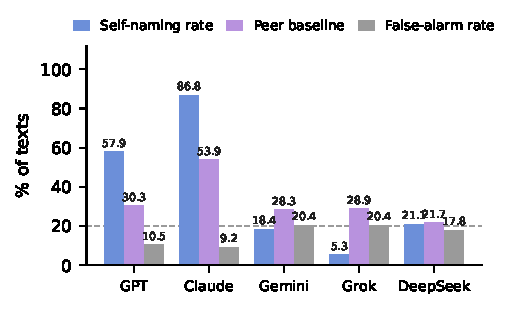
\includegraphics[width=\linewidth]{figures/lead_lineup.pdf}
\caption{Lineup of five answers}\label{fig:lead-lineup}
\end{subfigure}\hfill
\begin{subfigure}[b]{0.49\linewidth}\centering
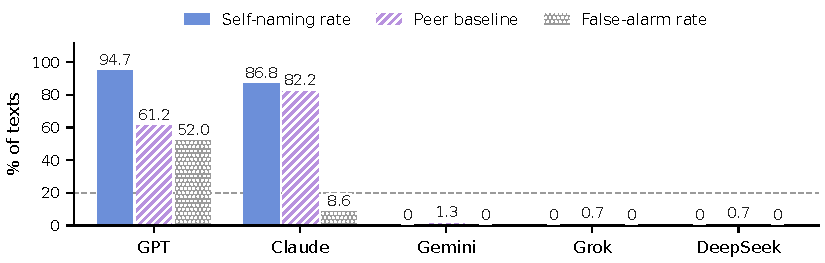
\includegraphics[width=\linewidth]{figures/lead_single.pdf}
\caption{One text at a time}\label{fig:lead-single}
\end{subfigure}
\caption{Figure~\ref{fig:lead-lineup} shows, for five frontier judges and 38
chat-app essays each, how often a judge names itself on its own essays
(self-naming rate), how often the other judges name it on those essays (peer
baseline), and how often it names itself on essays it did not write
(false-alarm rate). Claude and GPT beat their peers by 33 and 28 points; Grok
trails its peers. Figure~\ref{fig:lead-single} shows the same essays judged one
at a time: three judges never name themselves, GPT names itself on half of the
essays it did not write, and Claude's peers name Claude almost as often as
Claude does. The dashed line is the 20\% chance level.}
\label{fig:lead}
\end{figure}

Self-recognition is usually measured with one number: how often a judge names
itself as the author of its own text, compared with chance. We call this the
\emph{self-naming rate}, and we argue that it cannot answer the question on
its own. A judge that names itself on 87\% of its own answers may recognise
its writing. But the text may also be easy for \emph{any} model to attribute,
or the judge may simply say ``me'' to everything. The first case is a real
leak; the other two are not. Two further numbers from the same experiment tell
them apart: the \emph{false-alarm rate}, how often the judge names itself on
text it did not write, and the \emph{peer baseline}, how often the other judges
name it on its text (Figure~\ref{fig:lead}).

Prior evidence on self-recognition is contradictory.
\citet{panickssery2024selfpreference} report that models can recognise their
own outputs and link this to self-preference, while
\citet{davidson2024anonymized} find no consistent self-recognition in
anonymised panels, and \citet{bai2025selfrecognition} find accuracy near chance
when ten models are shown one text at a time. \citet{barkhordar2026stylenotself}
show for code that attribution accuracy mostly reflects how readily a model
claims authorship. These studies differ in models, texts and question formats,
and none compares a judge with how often \emph{other} judges attribute the same
text to it, so their conclusions are hard to reconcile.

To address this, we conduct a cross-evaluation study in which every model
serves as both author and judge. We evaluate nine judges, five frontier models
and four open-weight models, on three sets of texts: 190 essays the frontier
models wrote in their chat apps, 600 texts they wrote through the API in four
genres, and 480 texts the open-weight models wrote for the same 120 prompts.
Judges attribute the texts in three formats: a \emph{lineup} of answers to the
same prompt, \emph{one text at a time}, and the direct question ``Did you write
this text?''. In total we collect more than 19,000 authorship judgments.

Our findings reveal that most apparent self-recognition does not survive a peer
baseline. The usual test finds self-recognition in \SVPStd{} of \SVPCells{}
combinations of judge, text set and format; only \SVPProper{} pass our test,
which requires a judge both to beat its peers and to name itself more on its own
text than on others'. The cases that survive are large: in the lineup, Claude's
self-advantage over its peers is \ClaudeAdvLineup{} points \ClaudeAdvLineupCI{}
and GPT's is \GPTAdvLineup{} \GPTAdvLineupCI{}. Yet on 600 API texts from the same models no
judge beats its peers. The format alone reshapes the results. One text at a
time, judges send \SingleConcentration{} of all guesses to GPT or Claude, and
asked directly, GPT, Grok and DeepSeek deny writing any of the 190 essays,
their own included, a pattern we call \emph{self-denial}. Open-weight judges
show the opposite, \emph{over-attribution}: Llama names itself on every text it
is shown one at a time.

To understand these failures, we test what the judges rely on. The signal they
would need is present: a classifier over 18 style features attributes
\EngineAAcc{} of the essays, and each open-weight judge finds its own text the
most likely one on every prompt. Yet the judges' answers follow neither their
own likelihoods, nor the similarity of a text to their own writing, nor its
quality. With each essay's words shuffled, a bag-of-words classifier still
attributes \BowShufAcc{} while the judges fall to chance. Their stated reasons
reveal stereotypes of each model that they apply to every text alike.

In summary, we show that the standard test of LLM self-recognition is
unreliable, and we provide a corrected test that needs no data beyond what a
lineup already collects. Self-recognition, where it exists, is a property of a
particular judge on particular texts in a particular format, not a fixed trait
of a model. Anonymised evaluation should therefore be audited per judge, on the
texts it will actually judge, against a peer baseline.

\section{Additional Related Work}
\label{sec:related}

In this section, we provide additional context on self-preference in LLM
judges, prior measurements of self-recognition, and attribution of text to
models.

\paragraph{Self-preference in LLM judges}
LLM judges rate their own outputs above others'
\citep{panickssery2024selfpreference, wataoka2024perplexity, ye2025justice},
and their biases shift with format and position \citep{shi2025positionbias,
roytburg2026narcissists}. \citet{panickssery2024selfpreference} tie this
preference to self-recognition through fine-tuning, and
\citet{wataoka2024perplexity} to familiarity: judges favour text that is
predictable to them, which their own text usually is. CALM \citep{ye2025justice}
scores self-enhancement against the scores other judges give the same answer, a
peer reference for quality; we apply the same idea to authorship.

\paragraph{Empirical results on self-recognition}
Existing evidence is mixed. \citet{ackerman2025inspection} locate a
self-recognition direction in Llama-3-8B-Instruct, and \citet{zhou2025implicit}
find that models recognise their own text in pairs but not alone.
\citet{davidson2024anonymized} find no consistent self-recognition in
anonymised panels, \citet{bai2025selfrecognition} find accuracy near chance with
predictions concentrated on GPT and Claude, and \citet{laine2024sad} include
self-recognition in a situational-awareness benchmark.
\citet{stamand2026sgtr} show that picking the better text as one's own can
masquerade as self-recognition, and \citet{barkhordar2026stylenotself} show for
code that raw accuracy mostly reflects how readily a model claims authorship.
We extend this line of work with a peer baseline, a comparison of question
formats on identical texts, four genres, and likelihoods for open-weight
judges. \citet{khullar2026selfattribution} show that a monitor rates its own
earlier actions more favourably within a conversation; our answer-first
condition tests whether that position also helps a judge recognise its writing.

\paragraph{Attributing text to models}
Supervised classifiers separate model families with high accuracy
\citep{sun2025stylometric, bitton2025fingerprints, rosenfeld2026whose,
zaitsu2025stylometry, russell2026storyscope}, even after the words of each text
are shuffled \citep{sun2025stylometric}, and few-shot LLM judges can approach
classifier accuracy \citep{dietrich2026splits}. We study the zero-shot case,
which is how anonymised judging pipelines use judges.

\paragraph{Watermarks}
Text watermarks bias token choices using a secret key
\citep{kirchenbauer2023watermark, dathathri2024synthid}. Google marks text from
the Gemini app with SynthID-Text, and Anthropic announced watermarking of Claude
text in August 2026 \citep{anthropic2026watermark}. We discuss whether judges
could be reading a watermark in Section~\ref{sec:mechanism}.

\section{Measuring Self-Recognition}
\label{sec:measure}

A \emph{panel} is a set of models that both write texts and judge them, so
each judge sees some texts of its own among the texts it judges. For each
judge we compute three rates from the same set of judgments:
\begin{itemize}
\item \textbf{self-naming rate}: the share of the judge's own texts that it
says it wrote;
\item \textbf{false-alarm rate}: the share of other models' texts that it
says it wrote;
\item \textbf{peer baseline}: the share of the judge's texts that the
\emph{other} judges attribute to it.
\end{itemize}
From these we take two differences. \textbf{Discrimination} is the
self-naming rate minus the false-alarm rate: does the judge claim its own
text more than others'? \textbf{Self-advantage} is the self-naming rate minus
the peer baseline: does the judge know its own text better than other judges
do? With five candidate authors, guessing at random gives 20\% for all three
rates and zero for both differences.

\paragraph{Two tests} The \emph{usual test} asks only whether the
self-naming rate is above chance. \emph{Our test} requires both a
self-advantage and discrimination. Discrimination alone already means
anonymisation fails for that judge; the self-advantage shows whether the
judge has any special knowledge of its own writing, beyond what any judge
could see.

\paragraph{An example} In the lineup (Section~\ref{sec:frontier}), Claude
names itself on 33 of its 38 texts (87\%) and on only 14 of the 152 texts it
did not write (9\%). The other four judges name Claude on 54\% of Claude's
texts. Claude discriminates and beats its peers by 33 points, so it passes.
Shown the same texts one at a time, Claude still names itself on 33 of 38.
But now its peers name Claude on 82\% of Claude's texts, because in this
format every judge names Claude or GPT for almost everything. Claude's
self-naming rate is unchanged, yet its self-advantage nearly disappears. In
the same format GPT names itself on 36 of its 38 texts, the highest rate in
the study, but also on 79 of the 152 texts it did not write. The self-naming
rate alone cannot tell these cases apart.

\paragraph{Statistics} Judgments of the same prompt are not independent,
since every judge sees the same few texts. All our tests therefore resample
or shuffle whole prompts or whole texts, never single judgments: 95\%
intervals come from resampling prompts, and $p$-values from permutation
tests (shuffling which judge counts as ``self'' on each text, or which text
in a lineup is the judge's own). We correct for testing several judges at
once with Holm's method. For yes/no questions answered with a probability,
we report the AUC, which does not depend on how readily a judge says yes.
Appendix~\ref{app:stats} gives details.

\section{Experimental Setup}
\label{sec:setup}

\begin{table}[t]
\centering\small
\begin{adjustbox}{max width=\linewidth}
\begin{tabular}{l l r l r l}
\toprule
Texts & Written by & Prompts & Genres & Texts & Formats judged \\
\midrule
Chat-app essays & 5 frontier models, chat apps & 38 & essays & 190 & lineup, one text, yes/no \\
API texts & 5 frontier models, API & 120 & all four & 600 & lineup, one text \\
Open-weight texts & 4 open-weight models & 120 & all four & 480 & lineup, one text, yes/no \\
\bottomrule
\end{tabular}
\end{adjustbox}
\caption{The three sets of texts. The 38 chat-app prompts are among the 120;
all 120 are in the repository (\texttt{data/prompts\_v2.csv}), with one
example per genre in Appendix~\ref{app:data}. In each set, the models that wrote the texts also judge them; the chat-app essays carry the product labels listed in Section~\ref{sec:setup}.}
\label{tab:data}
\end{table}


\subsection{Texts}

We use three sets of texts, summarised in Table~\ref{tab:data}. All are built
from one bank of prompts designed so that answers to the same prompt differ
mainly in style: each prompt fixes the topic and the points the answer must
cover, and essay prompts ask for plain paragraphs with no lists, headers or
bold (Appendix~\ref{app:data} gives an example of each genre).

\paragraph{Chat-app essays} Five frontier models, GPT-5.5, Claude Opus
4.7, Gemini 3.5 Flash, Grok 4.3 and DeepSeek's chat model, each answered 39
argumentative prompts in their consumer chat apps at default settings,
between 15 June and 31 July 2026. One prompt was dropped because two of its
answers were corrupted copies, leaving 38 prompts and 190 essays.

\paragraph{API texts} To test whether results hold beyond one small set of
essays, the same five models answered 120 prompts through the API on 1
October 2026 (temperature 0.7, no system prompt): 60 essays (including the 38
above), 20 Python functions, 20 short explanations and 20 math word problems,
giving 600 texts.

\paragraph{Open-weight texts} Four open-weight models, Qwen2.5-7B
(Alibaba), Llama-3.1-8B (Meta), Mistral-7B-v0.3 (Mistral AI) and Phi-4-mini
(Microsoft), answered the same 120 prompts (temperature 0.7), giving 480
texts, plus a second, independent answer to every prompt. We generated these
texts ourselves from public weights, so none carries a watermark.

\subsection{Judges}

In each set, the models that wrote the texts are the judges, so ``self''
always means the same model on both sides. The frontier models judge through
OpenRouter at temperature~0.\footnote{Six of Claude's 38 chat-app essays were
written by Claude Sonnet 4.6 rather than Opus 4.7; dropping them leaves
Claude's lineup self-naming rate at 27 of 32 (84\%). The DeepSeek endpoint
could not be pinned to a snapshot.} The open-weight models run in 4-bit on a
single laptop GPU with greedy decoding (Appendix~\ref{app:openweight}). Judges
are never given examples, and see the prompt only in the answer-first
condition below. With five candidate
authors chance is 20\%; with four, 25\%.

\subsection{Question Formats}

Judges answer in the following formats; the exact instructions are in
Appendix~\ref{app:instructions}.
\begin{itemize}
\item \textbf{Lineup.} The judge sees all answers to one prompt, labelled A,
B, C, \ldots, and names an author for each. It is told it may name the same
model more than once, and the order of answers is balanced across judges.
\item \textbf{One text at a time.} The judge sees a single answer and names
its author from the panel.
\item \textbf{Yes/no.} The judge is asked ``Did you write this text?'' in a
fresh conversation. For open-weight judges we read the probability of
``yes''; no frontier provider returned probabilities, so for frontier judges
we use the answer itself.
\item \textbf{Answer first (open-weight only).} Following
\citet{khullar2026selfattribution}, the judge first answers the prompt
itself and is then asked the yes/no question about either that same answer, a
separate answer of its own, or a peer's answer.
\item \textbf{Shuffled lineup (frontier, chat-app essays only).} The lineup
again, with every essay's words shuffled, which keeps the vocabulary but
removes word order and structure.
\end{itemize}

\subsection{A Reference Classifier}

To measure how much the texts reveal about their authors, we train a random
forest on 18 simple style features (length, punctuation, vocabulary richness,
readability), always testing on prompts it was not trained on. It identifies
the author of \EngineAAcc{} of the chat-app essays (95\% CI \EngineACI{};
chance \Chance{}) and \OWClfPooled{} of the open-weight texts (chance 25\%),
more than any judge achieves (Appendix~\ref{app:classifier}).

\section{Results: Frontier Judges}
\label{sec:frontier}

\subsection{Chat-App Essays}

\begin{table}[t]
\centering\small\setlength\tabcolsep{3.5pt}
\begin{adjustbox}{max width=\linewidth}
\begin{tabular}{llrrrrrr}
\toprule
Format & Judge & Self-naming & False alarms & Peer baseline & Self-adv. [95\% CI] & $p$ (Holm) & Skill-adj. \\
\midrule
Lineup & GPT & 22/38 & 16/152 & 46/152 & +27.6 [+10.5, +44.7] & $0.008$ & +19.3 \\
 & Claude & 33/38 & 14/152 & 82/152 & +32.9 [+21.1, +44.1] & $0.002$ & +35.1 \\
 & Gemini & 7/38 & 31/152 & 43/152 & $-$9.9 [$-$23.0, +4.6] & $0.619$ & $-$19.3 \\
 & Grok & 2/38 & 31/152 & 44/152 & $-$23.7 [$-$32.9, $-$13.2] & $0.008$ & $-$20.2 \\
 & DeepSeek & 8/38 & 27/152 & 33/152 & $-$0.7 [$-$15.1, +15.1] & $1.000$ & +11.4 \\
\midrule
Single & GPT & 36/38 & 79/152 & 93/152 & +33.6 [+25.0, +42.1] & $2.1\times10^{-4}$ & -- \\
 & Claude & 33/38 & 13/152 & 125/152 & +4.6 [$-$7.2, +14.5] & $1.000$ & -- \\
 & Gemini & 0/38 & 0/152 & 2/152 & $-$1.3 [$-$3.3, +0.0] & $1.000$ & -- \\
 & Grok & 0/38 & 0/152 & 1/152 & $-$0.7 [$-$2.0, +0.0] & $1.000$ & -- \\
 & DeepSeek & 0/38 & 0/152 & 1/152 & $-$0.7 [$-$2.0, +0.0] & $1.000$ & -- \\
\bottomrule
\end{tabular}
\end{adjustbox}
\caption{Frontier judges on the chat-app essays. Self-naming: the judge names itself on its own 38 texts. False alarms: it names itself on the 152 texts it did not write. Peer baseline: the other four judges name it on its texts. Self-advantage is the difference in rates, with a prompt-bootstrap interval; $p$ is the exact within-response randomisation test, Holm-corrected over the five judges. Skill-adjusted removes each judge's general accuracy and each author's identifiability (Appendix~\ref{app:stats}); it is not interpretable in single-text, where a judge's accuracy mostly reflects which model it habitually names. In single-text, Gemini, Grok and DeepSeek never name themselves.}
\label{tab:frontier}
\end{table}


\paragraph{In the lineup, two judges recognise themselves and one does worse
than chance} Table~\ref{tab:frontier} reports every quantity from
Section~\ref{sec:measure}. Claude's self-advantage is \ClaudeAdvLineup{}
points \ClaudeAdvLineupCI{} and GPT's is \GPTAdvLineup{} \GPTAdvLineupCI{}.
Both keep false alarms near 10\%, so both also discriminate: these are genuine
leaks that anonymisation does not stop. DeepSeek and Gemini show no
advantage. Grok does significantly \emph{worse} on its own text than its peers
do (\GrokAdvLineup{} \GrokAdvLineupCI{}), naming itself on only 2 of its 38
essays. The verdicts for Claude, GPT and Grok hold under every analysis we
tried, including mixed-effects models and an adjustment for each judge's
general skill at attribution (Appendix~\ref{app:stats}). Gemini's does not:
it is among the best at attributing \emph{other} models' text, so after that
adjustment it too trails its peers on its own.

\paragraph{One text at a time, the format sets the answer} Shown a single
text, the judges send \SingleConcentration{} of all 950 guesses to GPT or
Claude, consistent with \citet{bai2025selfrecognition}. Gemini, Grok and
DeepSeek never name themselves at all, so for them this format measures
nothing. GPT's self-naming rate rises to \GPTSelfSingle{}, but it also names
itself on half the texts it did not write. Claude keeps its self-naming rate
(\ClaudeSelfSingle{}) but loses its self-advantage (\ClaudeAdvSingle{}),
because its peers now name Claude on \ClaudePeerSingle{} of Claude's texts.
The same texts and judges thus yield a very different picture, and the peer
baseline is informative only when judges spread their guesses.

\subsection{Asking Directly}
\label{sec:frontiernew}

\begin{table}[t]
\centering\small
\setlength\tabcolsep{3pt}
\begin{adjustbox}{max width=\linewidth}
\begin{tabular}{l rr r l r}
\toprule
Judge & Hits & False alarms & Hit$-$FA & AUC [95\% CI] & $p$ (Holm) \\
\midrule
GPT & 0/38 & 0/152 & +0.0 & 0.50 [0.50, 0.50] & $1.000$ \\
Claude & 28/38 & 76/152 & +23.7$^{*}$ & 0.62 [0.53, 0.70] & $0.037$ \\
Gemini & 0/38 & 2/152 & $-$1.3 & 0.49 [0.48, 0.50] & $1.000$ \\
Grok & 0/38 & 0/152 & +0.0 & 0.50 [0.50, 0.50] & $1.000$ \\
DeepSeek & 0/38 & 0/152 & +0.0 & 0.50 [0.50, 0.50] & $1.000$ \\
\bottomrule
\end{tabular}
\end{adjustbox}
\caption{Frontier judges asked ``Did you write this text?'' about each of the 190 chat-app essays in a fresh conversation (38 own and 152 others' per judge). Hits: yes to its own essays; false alarms: yes to others'. No provider returned probabilities, so the AUC is computed from the yes/no answers. $p$ is corrected for the five judges; $^{*}p<0.05$.}
\label{tab:fyesno}
\end{table}


We next asked each judge, about each of the 190 essays and in a fresh
conversation, ``Did you write this text?'' (Table~\ref{tab:fyesno}). GPT,
Grok and DeepSeek answered ``No'' to all 190, including their own 38. Gemini
said yes twice, both times to text it did not write. Only Claude ever claims
its own text: it says yes to \FBClaudeHitK{} of its own essays and to
\FBClaudeFAK{} of the others', so it discriminates (\FBClaudeDisc{} points,
Holm $p=$~\FBClaudeHolm{}) while also claiming half of what it did not write.
Strikingly, GPT, which names itself on 95\% of its own essays when it has five
names to choose from, never claims one when asked directly. The question, not
the text, determines the answer.

\subsection{Shuffling the Words}

% Shuffled-lineup table, corrected (issue I15). Numbers hard-coded; recomputed from
% repo/results/revision/frontier/shuffle_lineup.jsonl by work/verify-I15/t8.py.
% SAMPLE RULE (applies to every cell of every row): the 24 prompts on which all
% four answering judges (GPT, Gemini, Grok, DeepSeek) returned a complete,
% parseable shuffled lineup (ok = true). That is 96 lineups and 480 judgments.
%   Self   = judge names itself on its own essay, k/24
%   Peer   = the three other answering judges name it on its essay, k/72
%            (Claude has no shuffled judgments, so it is not a peer)
%   FA     = judge names itself on the four essays it did not write, k/96
%   Self-adv. = Self - Peer; percentile bootstrap over the 24 prompts
%   Hit-FA = Self - FA (now equals the printed Self minus the printed FA)
% Counts: GPT 9/24, 18/72, 15/96; Gemini 5/24, 13/72, 19/96;
%         Grok 2/24, 10/72, 22/96; DeepSeek 3/24, 7/72, 21/96.
% Exact randomisation p (uncorrected / Holm over four judges):
%   Self-adv.: GPT 0.31/1.00, Gemini 1.00/1.00, Grok 0.67/1.00, DeepSeek 1.00/1.00
%   Hit-FA:    GPT 0.041/0.16, Gemini 1.00/1.00, Grok 0.20/0.61, DeepSeek 0.45/0.91
% The earlier version took Self and Peer from these 24 prompts but FA and Hit-FA
% from all 38 (GPT 17.1%, +14.5; Grok 21.7%, -8.6; DeepSeek 21.7%, -8.6).
% Original (last column) is unchanged: unshuffled essays, all 38 prompts, four peers.
\begin{table}[t]
\centering\small
\setlength\tabcolsep{2.5pt}
\begin{adjustbox}{max width=\linewidth}
\begin{tabular}{l rrr l r r}
\toprule
Judge & Self & Peer & FA & Self-adv. [95\% CI] & Hit$-$FA & Original \\
\midrule
GPT & 37.5\% & 25.0\% & 15.6\% & +12.5 [$-$12.5, +38.9] & +21.9 & \GPTAdvLineup \\
Claude & \multicolumn{5}{c}{\emph{refused every lineup}} & \ClaudeAdvLineup \\
Gemini & 20.8\% & 18.1\% & 19.8\% & +2.8 [$-$15.3, +22.2] & +1.0 & \GeminiAdvLineup \\
Grok & 8.3\% & 13.9\% & 22.9\% & $-$5.6 [$-$16.7, +6.9] & $-$14.6 & \GrokAdvLineup \\
DeepSeek & 12.5\% & 9.7\% & 21.9\% & +2.8 [$-$11.1, +19.4] & $-$9.4 & \DeepSeekAdvLineup \\
\bottomrule
\end{tabular}
\end{adjustbox}
\caption{The chat-app lineup repeated with every essay's words shuffled. All columns use the 24 prompts on which GPT, Gemini, Grok and DeepSeek each returned a complete lineup (Gemini returned none for 14 of the 38). Columns as in Table~\ref{tab:frontier}, with the peer baseline taken over the three other answering judges; Original is the self-advantage on the unshuffled essays (all 38 prompts, four peers). Claude's provider refused all 38 of Claude's shuffled lineups, so Claude has no judgments here and is not a peer, although its essays stayed in every lineup. No value is significant after Holm correction over the four judges (smallest corrected $p=0.16$, for GPT's Hit$-$FA).}
\label{tab:fshuffle}
\end{table}


Do the judges rely on word choice, or on word order and structure? We
repeated the lineup with every essay's words shuffled, which preserves the
vocabulary and punctuation but destroys sentences and paragraphs. Claude's
provider refused all 38 of Claude's shuffled lineups with a content filter (a
repeat on Anthropic's own endpoint was also refused), and Gemini gave no answer
on \FSGeminiMissing{} of its 38; we treat both as missing. The remaining
judges fall to chance (accuracy \FSAcc{}; Table~\ref{tab:fshuffle}), and no
self-advantage or discrimination is significant. Yet the word distribution
alone still identifies the author: a bag-of-words classifier attributes
\BowShufAcc{} of the shuffled essays, in line with \citet{sun2025stylometric}.
The judges depend on reading the text as prose and do not exploit the word
statistics that a classifier uses.

\subsection{A Larger and More Varied Set of Texts}
\label{sec:frontier120}

\begin{table}[t]
\centering\small
\setlength\tabcolsep{2.5pt}
\begin{adjustbox}{max width=\linewidth}
\begin{tabular}{l rrr rr}
\toprule
Judge & Self & Peer & FA & Self-adv. [95\% CI] & Hit$-$FA \\
\midrule
\multicolumn{6}{l}{\emph{Lineup}} \\
GPT & 19.2\% & 15.0\% & 20.4\% & +4.2 [$-$3.3, +12.1] & $-$1.2 \\
Claude & 56.7\% & 50.4\% & 12.7\% & +6.2 [$-$2.5, +14.8] & +44.0$^{*}$ \\
Gemini & 26.7\% & 31.9\% & 18.3\% & $-$5.2 [$-$14.4, +3.8] & +8.3 \\
Grok & 32.5\% & 30.2\% & 16.2\% & +2.3 [$-$7.1, +11.9] & +16.2$^{*}$ \\
DeepSeek & 21.7\% & 18.8\% & 17.7\% & +2.9 [$-$5.2, +11.5] & +4.0 \\
\midrule
\multicolumn{6}{l}{\emph{One text at a time}} \\
GPT & 83.3\% & 63.1\% & 84.4\% & +20.2$^{*}$ [+13.5, +26.7] & $-$1.0 \\
Claude & 40.8\% & 49.8\% & 3.1\% & $-$9.0 [$-$16.0, $-$1.5] & +37.7$^{*}$ \\
Gemini & 8.3\% & 4.0\% & 4.8\% & +4.4 [$-$0.4, +9.6] & +3.5 \\
Grok & 1.7\% & 0.0\% & 0.6\% & +1.7 [+0.0, +4.2] & +1.0 \\
DeepSeek & 0.0\% & 10.6\% & 0.0\% & $-$10.6$^{*}$ [$-$12.9, $-$8.3] & +0.0 \\
\bottomrule
\end{tabular}
\end{adjustbox}
\caption{The five frontier judges on 600 texts the same five models wrote through the API for 120 prompts in four genres (120 own texts per judge). Columns as in Table~\ref{tab:frontier}; $^{*}$Holm-corrected within-prompt permutation $p<0.05$.}
\label{tab:frontier120}
\end{table}


Thirty-eight essays per judge is a small sample from a single genre. We
therefore repeat the lineup and one-text formats on the 600 API texts in four
genres (Table~\ref{tab:frontier120}).

\paragraph{No judge beats its peers, but Claude still discriminates} In the
lineup, no self-advantage is significant. Claude names itself on
\FXClaudeLineupSelf{} of its own texts and only \FXClaudeLineupFA{} of others'
(discrimination \FXClaudeLineupDisc{} points), but its peers now name Claude on
\FXClaudeLineupPeer{} of its texts, almost as often. Grok, which trailed its
peers on the chat-app essays, now discriminates too (\FXGrokLineupDisc{}). One
text at a time, the judges again send \FXSingleTopTwo{} of their guesses to GPT
or Claude, and GPT names itself on \FXGPTSingleNamesSelf{} of all texts,
whoever wrote them.

\paragraph{What changed} The API texts differ from the chat-app essays in
collection channel, decoding, date and genre. On the 38 prompts the two sets
share, Claude's and GPT's self-advantages keep their sign but shrink
(\FXOldClaudeLineupAdv{} and \FXOldGPTLineupAdv{} points) and are no longer
significant; Claude's peers name its API essays more often. On the 82 new
prompts no judge's self-advantage reaches 10 points, while Claude's
discrimination holds. By genre, Claude's discrimination is largest on essays
and absent on math, where answers to the same problem share most of their
words (Appendix~\ref{app:more}).

\begin{takeaway}
\textbf{Takeaway.} Genuine self-recognition exists among frontier judges
(Claude and GPT beat their peers by 33 and 28 points on essays), but it does
not carry over to a second set of texts from the same models, and the question
format alone can create it, hide it, or reverse it.
\end{takeaway}

\section{Open-weight judges}
\label{sec:openweight}

The frontier study has three limits: closed models whose probabilities we
cannot read, vendors that may watermark their text, and few genres. We
repeat it with four smaller open-weight models, which avoid all three but are
much weaker judges, so this study says little about frontier models directly.

\subsection{Setup}

\paragraph{Panel and texts.} Qwen2.5-7B (Alibaba), Llama-3.1-8B (Meta),
Mistral-7B-v0.3 (Mistral AI) and Phi-4-mini (Microsoft), each run in 4-bit on
a single laptop GPU (Appendix~\ref{app:openweight}). With four candidates,
chance is 25\%. Each model answered the same 120 prompts as the API texts
(temperature 0.7), giving 480 texts, plus a second, independent answer to
every prompt. We generated the texts ourselves from public weights, so none
carries a watermark.

\paragraph{Formats.} The judges use the lineup and one-text formats with
their own four names, and answer ``Did you write this text?'' about every
text in a fresh conversation. Here we read the probability of ``yes'' from
the model, so we can compute an AUC. Two further conditions follow
\citet{khullar2026selfattribution}: the judge first answers the prompt
itself and is then asked the yes/no question about a candidate answer
(Section~\ref{sec:onpolicy}). We also read each judge's likelihood of every
text, and had each judge rate every text's quality (Section~\ref{sec:mechanism}).

\subsection{Results}

\begin{table*}[t]
\centering\small
\setlength\tabcolsep{3.5pt}
\begin{tabular}{l rrrrr rrr rr}
\toprule
 & \multicolumn{5}{c}{Lineup} & \multicolumn{3}{c}{Yes/no, fresh context} & \multicolumn{2}{c}{Own likelihood} \\
\cmidrule(lr){2-6}\cmidrule(lr){7-9}\cmidrule(lr){10-11}
Judge & Self & Peer & FA & Self-adv. [95\% CI] & Hit$-$FA & Hit & FA & AUC & Pick-self & AUC \\
\midrule
Qwen & 56.7\% & 15.8\% & 49.2\% & +40.8$^{*}$ [+31.1, +50.6] & +7.5 & 51.7\% & 58.6\% & 0.45 & 100.0\% & 1.00 \\
Llama & 32.5\% & 22.2\% & 36.1\% & +10.3$^{*}$ [+1.9, +18.6] & $-$3.6 & 85.8\% & 85.6\% & 0.53 & 100.0\% & 1.00 \\
Mistral & 25.0\% & 20.8\% & 20.3\% & +4.2 [$-$6.1, +14.4] & +4.7 & 99.2\% & 99.4\% & 0.41$^{*}$ & 100.0\% & 1.00 \\
Phi & 20.8\% & 22.8\% & 22.5\% & $-$1.9 [$-$10.6, +6.9] & $-$1.7 & 4.2\% & 1.4\% & 0.53 & 100.0\% & 1.00 \\
\bottomrule
\end{tabular}
\caption{Open-weight judges, all four genres pooled (120 prompts). Lineup: self-naming, peer-baseline and false-alarm (FA) rates, the self-advantage with a prompt-bootstrap interval, and the hit minus false-alarm rate, which is positive only if a judge names itself more on its own text than on others'. Yes/no: ``Did you write this text?'' in a fresh context; hit and false-alarm rates at $P(\text{yes})>0.5$ and the AUC of $P(\text{yes})$ for own versus others' text (0.5 is chance). Own likelihood: the share of prompts on which the text the judge finds most likely, relative to the other judges, is its own (chance 25\%), and the AUC of that relative likelihood. $^{*}$Holm-corrected within-prompt permutation $p<0.05$ across the four judges.}
\label{tab:openweight}
\end{table*}


\paragraph{No open-weight judge recognises itself in the lineup.} Qwen and
Llama beat their peers (Table~\ref{tab:openweight}), but neither
discriminates. Qwen names itself on \OWQwenLineupSelf{} of its own texts, but
also on \OWQwenLineupFA{} of the texts it did not write; Llama names itself
\emph{more} often on others' texts than on its own. Both put their own name on
much of what they read, which is enough to beat peers who rarely name them.
Overall lineup accuracy is \OWLineupAcc{}, at chance, even though a style
classifier attributes these texts at \OWClfPooled{}.

\paragraph{One text at a time, and asked directly, each judge answers by
habit.} Shown one text at a time, Qwen names itself on \OWQwenSingleNamesSelf{}
of all texts and Llama on every text, whoever wrote them; all four judges have
a significant self-advantage and none discriminates
(Appendix~\ref{app:more}). Asked ``Did you write this text?'', Mistral says
yes to \OWMistralBinaryHit{} of its own texts and \OWMistralBinaryFA{} of
everyone else's, while Phi says yes to \OWPhiBinaryHit{} and
\OWPhiBinaryFA{}. Read as self-naming rates, these would rank the judges from
near-certain self-recognition to none. The AUC, which ignores how readily a
judge says yes, is at or below chance for all four (0.41 to 0.53); Mistral's
is reliably \emph{below} chance.

\subsection{Answering the task first}
\label{sec:onpolicy}

\begin{table}[t]
\centering\small
\setlength\tabcolsep{4pt}
\begin{adjustbox}{max width=\linewidth}
\begin{tabular}{l rrl rrl rrl}
\toprule
 & \multicolumn{3}{c}{Asked in a fresh conversation} & \multicolumn{3}{c}{After answering: same answer} & \multicolumn{3}{c}{After answering: a new answer} \\
\cmidrule(lr){2-4}\cmidrule(lr){5-7}\cmidrule(lr){8-10}
Judge & Hit & FA & AUC [95\% CI] & Hit & FA & AUC [95\% CI] & Hit & FA & AUC [95\% CI] \\
\midrule
Qwen & \OWQwenBinaryHit & \OWQwenBinaryFA & \OWQwenBinaryAUC{} \OWQwenBinaryAUCCI & \OWQwenOnPolHit & \OWQwenOnPolFA & \OWQwenOnPolAUC{} \OWQwenOnPolAUCCI & \OWQwenOnPolResHit & \OWQwenOnPolResFA & \OWQwenOnPolResAUC{} \OWQwenOnPolResAUCCI \\
Llama & \OWLlamaBinaryHit & \OWLlamaBinaryFA & \OWLlamaBinaryAUC{} \OWLlamaBinaryAUCCI & \OWLlamaOnPolHit & \OWLlamaOnPolFA & \OWLlamaOnPolAUC{} \OWLlamaOnPolAUCCI & \OWLlamaOnPolResHit & \OWLlamaOnPolResFA & \OWLlamaOnPolResAUC{} \OWLlamaOnPolResAUCCI \\
Mistral & \OWMistralBinaryHit & \OWMistralBinaryFA & \OWMistralBinaryAUC{} \OWMistralBinaryAUCCI & \OWMistralOnPolHit & \OWMistralOnPolFA & \OWMistralOnPolAUC{} \OWMistralOnPolAUCCI & \OWMistralOnPolResHit & \OWMistralOnPolResFA & \OWMistralOnPolResAUC{} \OWMistralOnPolResAUCCI \\
Phi & \OWPhiBinaryHit & \OWPhiBinaryFA & \OWPhiBinaryAUC{} \OWPhiBinaryAUCCI & \OWPhiOnPolHit & \OWPhiOnPolFA & \OWPhiOnPolAUC{} \OWPhiOnPolAUCCI & \OWPhiOnPolResHit & \OWPhiOnPolResFA & \OWPhiOnPolResAUC{} \OWPhiOnPolResAUCCI \\
\bottomrule
\end{tabular}
\end{adjustbox}
\caption{Open-weight judges asked ``Did you write this text?'' (120 own and
360 other texts per judge and condition). Left: in a fresh conversation.
Middle: after answering the prompt, about either that same answer or a peer's.
Right: after answering the prompt, about either a separate answer of its own
or a peer's. Hit and false-alarm rates count a probability of ``yes'' above
0.5; the AUC uses the probability itself (0.5 is chance).}
\label{tab:owyesno}
\end{table}


\citet{khullar2026selfattribution} find that a monitor's judgment shifts most
when it evaluates something it produced earlier in the same conversation.
Does that position help a judge recognise its writing? In the
\emph{verbatim} condition the judge answers the prompt and is then shown
either that same answer, word for word, or a peer's answer. Every judge's
AUC is now above chance (Table~\ref{tab:owyesno}), but this is a low bar,
since the candidate is a copy of text already in the conversation; Llama's
AUC is only \OWLlamaOnPolAUC{}. In the \emph{resampled} condition the judge's
own turn is a fresh answer and the candidate is its other answer or a peer's,
so recognising it requires recognising its style rather than a copy. Qwen
and Phi now tell their own answer from peers' (AUC \OWQwenOnPolResAUC{} and
\OWPhiOnPolResAUC{}), while Llama and Mistral fall reliably \emph{below}
chance (\OWLlamaOnPolResAUC{} and \OWMistralOnPolResAUC{}). Seeing its own
answer to the task helps two judges and misleads the other two.

\section{What Judges Use to Attribute Text}
\label{sec:mechanism}
\label{sec:watermark}

Most cases do not pass both controls, and those that pass are all on the
chat-app essays. We consider five possible explanations for how the judges
attribute texts:
\begin{itemize}
\item the texts contain too little information about their authors;
\item judges claim texts similar to what they would have written;
\item judges claim texts that are likely under their own model, the familiarity
that \citet{wataoka2024perplexity} relate to self-preference;
\item judges claim the texts they consider best
\citep{davidson2024anonymized, stamand2026sgtr};
\item judges detect a watermark added by their developer.
\end{itemize}

\paragraph{Information in the texts}
A random forest over 18 style features attributes \EngineAAcc{} of the chat-app
essays (95\% CI \EngineACI{}) and \OWClfPooled{} of the open-weight texts, more
than any judge. To test whether the judges can attribute an essay from its
vocabulary alone, we repeated the lineup with the words of each essay
shuffled. Claude's provider refused all 38 of Claude's shuffled lineups, and
Gemini returned no usable answer for \FSGeminiMissing{} of its 38
(Appendix~\ref{app:data}), so this condition covers four judges and omits the
judge with the largest self-advantage on the intact essays. On the \FSNLineups{} answered
lineups the four judges attribute \FSAcc{} of the essays correctly, compared
with \CXIntactAccFour{} for the same judges on the intact essays and 20\% by
chance (Figure~\ref{fig:shuffle} and Table~\ref{tab:fshuffle} in
Appendix~\ref{app:more}), and no self-advantage or discrimination is
significant. A bag-of-words classifier trained on labelled essays attributes
\BowShufAcc{} of them, consistent with \citet{sun2025stylometric}. Its input is
the same before and after shuffling, so this accuracy holds for both versions
by construction; it shows that vocabulary alone carries authorship information,
which the judges, who see no labelled examples, do not use. The condition
cannot show which cues the judges use on intact essays. Every reasoning trace
returned by Gemini and Grok describes the essays as scrambled
(Appendix~\ref{app:more}), so chance-level accuracy may reflect judges that
stop attributing when the text is visibly corrupted, and we do not interpret
it as evidence about word order.

\paragraph{Similarity to the judge's own answer}
For each frontier judge, we use its own answer to the same prompt as an
estimate of what it would have written, and test whether the judge names itself
more often on other models' texts that are similar to that answer. Across four
similarity measures (style features, word and character $n$-grams, and
function words), the pooled odds ratio per standard deviation of similarity is
between 0.89 and 1.04 in the lineup and between 0.91 and 1.09 one text at a
time, and every confidence interval includes 1. Of the 36 per-judge and pooled
tests, which are correlated, 1 reaches $p<0.05$. The per-judge tests use 13 to
79 self-attributions and cannot exclude odds ratios near 2. The same similarity
measures identify the true author in 74--79\% of cases, and the judges' answers
follow them only weakly. When judges are wrong in the lineup, the model they
name is the one whose answer is most similar to the text in 31.9\% of 630
errors, compared with 30.1\% under random reassignment, and one text at a time
the excess is similar (Appendix~\ref{app:more}). These excesses of 1 to 2
points are significant in a permutation test ($p\le 0.002$) that does not
account for the same essays recurring across judges.

\paragraph{Judge likelihoods}
For each open-weight judge and text, we compute the mean token log-probability
of the text under the judge. Conditioned on the original prompt, the judge's
own text is the most likely of the four candidates on
\OWLikCondRawMin{}--\OWLikCondRawMax{} of prompts (chance 25\%). This is
expected, since each text was sampled from its author. The judges did not see
the prompt in the lineup, one-text and yes/no formats; scored without it, the
judge's own text is the most likely on \OWLikUncRawMin{}--\OWLikUncRawMax{} of
prompts, with Qwen and Phi lowest. Subtracting the mean log-probability under
the other three judges, which no judge can compute, raises these shares to
\OWLikCondAccMin{} with the prompt and \OWLikUncAccMin{}--\OWLikUncAccMax{}
without it (Table~\ref{tab:owlik}). A judge's own probabilities therefore carry
authorship information, and this information is weaker when the prompt is
withheld. Among texts a judge did not write, we find no evidence that the texts
it claims have a higher relative likelihood than the texts it does not claim.
None of the \OWFamTests{} tests is significant after Holm correction, and the
only one with uncorrected $p<0.05$ (\OWFamMinWho{}; $p=$~\OWFamMinP{},
corrected \OWFamMinHolm{}) is in the opposite direction
(Appendix~\ref{app:more}). Five of the six tests in the one-text and yes/no
formats use 34 or fewer prompts and cannot exclude a moderate effect.

\paragraph{Text quality}
The four open-weight models rated every chat-app essay and every open-weight
text on a 1--9 scale. Frontier judges do not preferentially claim higher-rated
essays, and the lineup self-advantages of Claude, GPT and Grok remain
significant when quality is included as a covariate. Almost all frontier essays
receive ratings near the top of the scale, so this control is coarse. We
detect no self-preference in the open-weight judges. For each judge we take
the amount by which it rates its own texts above its peers' ratings of the
same texts, and subtract the same difference for texts by other authors. The result
is at most \OWQualSelfPrefMax{} points (Mistral, 95\% interval
\OWMistralQualSelfPrefCI{}) and at most \OWQwenQualSelfPref{} for the other
three judges. These ratings are compressed: \CXQualModalTop{} of the judges'
most likely ratings are 7, 8 or 9
(Appendix~\ref{app:openweight}), so a modest preference
could go undetected. No frontier judge rated any text, so we have no measure of
self-preference for the judges that pass both controls.

\paragraph{Watermarks}
The watermarking schemes we consider
\citep{kirchenbauer2023watermark, dathathri2024synthid} are detected with a
key or seeding function that the judges were not given. The chat-app essays
were written between 15 June and 31 July 2026, before Anthropic announced
watermarking of Claude text in August
\citep{anthropic2026watermark, anthropic2026marking}, so Claude's
self-advantage on these essays predates any announced Claude watermark. The
API texts were collected on 1 October 2026, after the announcement, so this
timing argument does not apply to them. On those texts no judge exceeds its
peer baseline in the lineup, and the other judges name Claude on its texts
almost as often as Claude does (\FXClaudeLineupPeer{} against
\FXClaudeLineupSelf{}), which a mark readable only by the author's model would
not produce. Text from the Gemini app is watermarked
\citep{deepmind2026synthid}, and Gemini does not recognise its own essays. The open-weight texts have no watermark, and the classifier attributes
\OWClfPooled{} of them. The shuffled lineup would also remove a watermark, but
because the judges are at chance in that condition, it does not distinguish
the two explanations.

\paragraph{Stated reasons}
Each frontier judgment includes a one-sentence reason, and we coded all 1,900
reasons (Appendix~\ref{app:rationales}). No reason refers to the judge itself
(for example, ``this is how I write''). Judges refer to every model, including
themselves, in the third person, and 95\% of one-text reasons cite a model's
typical style. The cited features are the same for correct and incorrect
self-attributions (Table~\ref{tab:reasons}): when Claude names itself one text at
a time, it cites hedging in 31 of 33 correct cases and in 12 of 13 incorrect
ones. Grok and Gemini attribute their own essays to Claude and describe Claude's
style as ``polished'' and ``elegant'', similar to the preference for frontier
model families reported by \citet{bai2025selfrecognition}. The reasons often
plausibly describe surface properties of the texts, but each judge applies the
same description of a model to all texts, so the reasons do not separate its
own texts from others'.

\section{Concluding Discussion}
\label{sec:conclusion}
\label{sec:recs}
\label{sec:limits}

Our study evaluates self-recognition in nine LLM judges across three sets of
texts and three question formats. The usual test, a self-naming rate above
chance, flags self-recognition in \SVPStd{} cases, and only \SVPProper{} survive
a peer baseline and a false-alarm rate. Where self-recognition does exist, it
is large and invisible to anyone who looks at only one format or one set of
texts: Claude and GPT beat their peers by 33 and 28 points on chat-app essays
but not on 600 API texts, and the question format alone produces self-denial in
some judges and over-attribution in others. The information a judge would need
to recognise itself is already in the text and in its own probabilities, yet
the judges' answers do not follow it. Our contribution is not to declare
anonymisation safe or broken, but to provide a test that separates the two and
can be applied to any judging pipeline.

\paragraph{Implications}
Self-recognition is not a fixed trait of a model that can be certified once. It
depends on the judge, the texts and the question, so a judge that passes an
audit on one benchmark may leak on another, and a model update may change the
answer. Much of the work on self-preference assumes that judges recognise
their own outputs; our results suggest that, for most judges, the preference
must come from elsewhere, consistent with \citet{davidson2024anonymized} and
\citet{bai2025selfrecognition}. For the judges that do recognise themselves,
however, anonymisation offers no protection, and the usual test cannot tell
these judges from the many that merely appear to.

\paragraph{Recommendations}
We recommend four practices. (1)~Report the self-naming rate together with the
false-alarm rate and the peer baseline, which come from the same experiment,
and claim self-recognition only if a judge both discriminates and beats its
peers. (2)~Prefer a lineup to the one-text format, in which judges collapse onto
one or two names; use a yes/no question only if a judge's answers vary.
(3)~Measure each judge on the kind of text it will judge, and repeat the audit
when the judge or the texts change. (4)~Do not infer the mechanism from the
judges' stated reasons, which are the same for right and wrong self-attributions.
Our released code implements this audit.

\paragraph{Future directions}
The gap between what the texts reveal and what judges use suggests that
self-recognition could grow quickly if judges learned to use stylistic or
likelihood cues, through training, few-shot examples \citep{dietrich2026splits}
or access to their own probabilities. Tracking self-recognition across model
versions is therefore as important as measuring it once. Our test extends
directly to other judging tasks, such as pairwise preference and safety
monitoring, and to longer and multilingual texts. Interpretability work on the
representations behind self-attribution \citep{ackerman2025inspection} could
show why some judges discriminate on some genres and not others.

\paragraph{Limitations}
The chat-app essays contain only 38 texts per judge, so their intervals are
wide; the API texts have 120 per judge. The open-weight judges are small (4--8
billion parameters, run in 4-bit) and much weaker than frontier models. No
frontier provider returned token probabilities, so the frontier yes/no results
are hard answers, and the likelihood, quality and answer-first analyses cover
the open-weight judges only. All texts are in English and every prompt fixes the
content of the answer. The chat-app essays were collected in consumer apps whose
hidden system prompts we cannot see. The coding of the judges' reasons was
checked against two LLM annotators, both instances of Claude, which is also a
judge. Finally, every result describes particular model versions at particular
dates in 2026; providers update models behind stable names, and the DeepSeek
endpoint could not be pinned.

\section*{Acknowledgments}
We thank Ryan Erlikhman for his work on an earlier version of this study.

\section*{Reproducibility Statement}
Section~\ref{sec:setup} describes how we built the texts and called the models,
Appendix~\ref{app:data} gives the collection details, and
Appendix~\ref{app:instructions} reproduces every instruction given to a judge.
All texts, prompts, judgments with their reasons, archived API responses,
open-weight likelihoods and quality ratings, and the analysis code are available
at \CodeURL{}. Every number in the paper is generated from those files, and none
of the analyses requires an API key.

\section*{Ethics Statement}
The study involves no human subjects or personal data: every text was written
by a language model in response to our prompts. The frontier texts were
collected through the providers' apps and APIs under their terms of use, and the
open-weight models were run under their licences. We name the judges that
recognise their own text so that practitioners can account for them; the
results describe specific model versions and should not be read as permanent
properties of a vendor's models.


\bibliographystyle{acl_natbib}
\bibliography{references}

\clearpage
\appendix
\section{Additional Results}
\label{app:more}

This appendix gives the full results for Sections~\ref{sec:results}
and~\ref{sec:mechanism}. Figure~\ref{fig:shuffle} and Table~\ref{tab:fshuffle}
give the frontier judges on the word-shuffled essays. Figure~\ref{fig:guess}
and Table~\ref{tab:blame} show how often each model is named and how accurate
each judge is on others' text. Table~\ref{tab:naming} gives how often each
judge names Claude and GPT, with false-alarm rates, and Table~\ref{tab:anchor}
repeats the lineup results with the lineups in listed order removed and with
the self-advantage stratified by position. Tables~\ref{tab:fxgenre}
and~\ref{tab:fxsplit} split the API texts by genre and by whether a prompt was
shared with the chat-app essays, and Table~\ref{tab:shared} compares the two
text sets on the shared prompts with intervals. Table~\ref{tab:owyesno} gives
the open-weight judges in the yes/no format, including the answer-first
condition, Table~\ref{tab:owsingle} gives them one text at a time,
Table~\ref{tab:genre} breaks the open-weight results down by genre, and
Table~\ref{tab:owlik} reports what the open-weight judges' likelihoods contain
and whether their claims follow them.

\paragraph{Similarity of the named model to the text} One text at a time, the
model a judge names is the one whose average style is closest to the text in
33.9\% of judgments for function words, 30.6\% for character $n$-grams and
30.3\% for word $n$-grams, compared with 31.5\%, 28.7\% and 29.1\% under random
reassignment.

\paragraph{Prompts used by the likelihood tests} The tests compare texts
within a prompt. In the lineup they use 61 to 96 prompts per judge, but five of the six tests in the
other two formats use 34 or fewer, because the judges claim nearly all or
nearly none of the texts, so those five cannot exclude a moderate effect.

\paragraph{Shuffled lineup} The instruction did not mention the reordering.
Every reasoning trace returned by Gemini and Grok (38 each) describes the
essays as scrambled, and every answered lineup assigns each of the five names
once.

\begin{figure}[!ht]
\centering
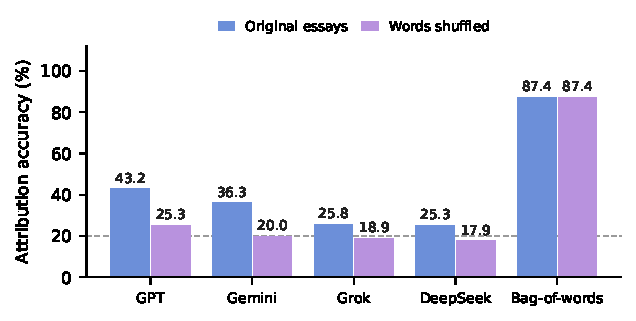
\includegraphics[width=0.8\linewidth]{figures/shuffle.pdf}
\caption{Lineup accuracy of four frontier judges on the chat-app essays in
their original form and with the words of each essay shuffled, compared with
a bag-of-words classifier on the same essays. With shuffled words the judges'
accuracy is between \FSDeepSeekOverall{} and \FSGPTOverall{}, close to chance
(dashed line). The classifier does not use word order, so its two bars are
equal by construction. Claude is omitted because its provider refused all
shuffled lineups, and Gemini's shuffled bar is based on 24 of its 38
lineups.}
\label{fig:shuffle}
\end{figure}

% Shuffled-lineup table, corrected (issue I15). Numbers hard-coded; recomputed from
% repo/results/revision/frontier/shuffle_lineup.jsonl by work/verify-I15/t8.py.
% SAMPLE RULE (applies to every cell of every row): the 24 prompts on which all
% four answering judges (GPT, Gemini, Grok, DeepSeek) returned a complete,
% parseable shuffled lineup (ok = true). That is 96 lineups and 480 judgments.
%   Self   = judge names itself on its own essay, k/24
%   Peer   = the three other answering judges name it on its essay, k/72
%            (Claude has no shuffled judgments, so it is not a peer)
%   FA     = judge names itself on the four essays it did not write, k/96
%   Self-adv. = Self - Peer; percentile bootstrap over the 24 prompts
%   Hit-FA = Self - FA (now equals the printed Self minus the printed FA)
% Counts: GPT 9/24, 18/72, 15/96; Gemini 5/24, 13/72, 19/96;
%         Grok 2/24, 10/72, 22/96; DeepSeek 3/24, 7/72, 21/96.
% Exact randomisation p (uncorrected / Holm over four judges):
%   Self-adv.: GPT 0.31/1.00, Gemini 1.00/1.00, Grok 0.67/1.00, DeepSeek 1.00/1.00
%   Hit-FA:    GPT 0.041/0.16, Gemini 1.00/1.00, Grok 0.20/0.61, DeepSeek 0.45/0.91
% The earlier version took Self and Peer from these 24 prompts but FA and Hit-FA
% from all 38 (GPT 17.1%, +14.5; Grok 21.7%, -8.6; DeepSeek 21.7%, -8.6).
% Original (last column) is unchanged: unshuffled essays, all 38 prompts, four peers.
\begin{table}[t]
\centering\small
\setlength\tabcolsep{2.5pt}
\begin{adjustbox}{max width=\linewidth}
\begin{tabular}{l rrr l r r}
\toprule
Judge & Self & Peer & FA & Self-adv. [95\% CI] & Hit$-$FA & Original \\
\midrule
GPT & 37.5\% & 25.0\% & 15.6\% & +12.5 [$-$12.5, +38.9] & +21.9 & \GPTAdvLineup \\
Claude & \multicolumn{5}{c}{\emph{refused every lineup}} & \ClaudeAdvLineup \\
Gemini & 20.8\% & 18.1\% & 19.8\% & +2.8 [$-$15.3, +22.2] & +1.0 & \GeminiAdvLineup \\
Grok & 8.3\% & 13.9\% & 22.9\% & $-$5.6 [$-$16.7, +6.9] & $-$14.6 & \GrokAdvLineup \\
DeepSeek & 12.5\% & 9.7\% & 21.9\% & +2.8 [$-$11.1, +19.4] & $-$9.4 & \DeepSeekAdvLineup \\
\bottomrule
\end{tabular}
\end{adjustbox}
\caption{The chat-app lineup repeated with every essay's words shuffled. All columns use the 24 prompts on which GPT, Gemini, Grok and DeepSeek each returned a complete lineup (Gemini returned none for 14 of the 38). Columns as in Table~\ref{tab:frontier}, with the peer baseline taken over the three other answering judges; Original is the self-advantage on the unshuffled essays (all 38 prompts, four peers). Claude's provider refused all 38 of Claude's shuffled lineups, so Claude has no judgments here and is not a peer, although its essays stayed in every lineup. No value is significant after Holm correction over the four judges (smallest corrected $p=0.16$, for GPT's Hit$-$FA).}
\label{tab:fshuffle}
\end{table}


\begin{figure}[!ht]
\centering
\begin{subfigure}[b]{0.49\linewidth}\centering
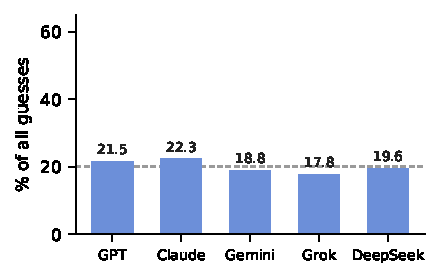
\includegraphics[width=\linewidth]{figures/guess_lineup.pdf}
\caption{Lineup}\label{fig:guess-lineup}
\end{subfigure}\hfill
\begin{subfigure}[b]{0.49\linewidth}\centering
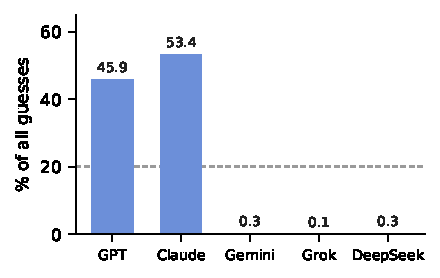
\includegraphics[width=\linewidth]{figures/guess_single.pdf}
\caption{One text at a time}\label{fig:guess-single}
\end{subfigure}
\caption{Share of the 950 attributions on the chat-app essays that name each
model. In the lineup the shares are close to uniform. One text at a time, GPT
and Claude receive \SingleConcentration{} of attributions and Gemini, Grok and
DeepSeek almost none. The dashed line marks a uniform distribution (20\%).}
\label{fig:guess}
\end{figure}

\begin{figure}[!ht]
\centering
\begin{subfigure}[b]{0.49\linewidth}\centering
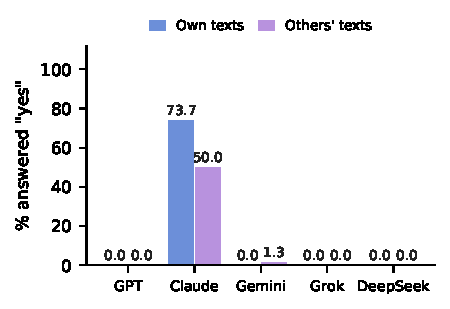
\includegraphics[width=\linewidth]{figures/yes_frontier.pdf}
\caption{Frontier judges, chat-app essays}\label{fig:yes-frontier}
\end{subfigure}\hfill
\begin{subfigure}[b]{0.49\linewidth}\centering
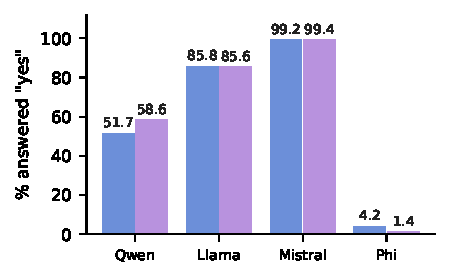
\includegraphics[width=\linewidth]{figures/yes_open.pdf}
\caption{Open-weight judges}\label{fig:yes-open}
\end{subfigure}
\caption{Share of texts for which a judge answers ``yes'' to ``Did you write
this text?'', separately for its own texts and for other models' texts.
(a) GPT, Grok and DeepSeek answer no for every essay; Claude is the only judge
that answers yes for its own essays. (b) Mistral answers yes for almost every
text and Phi for almost none, regardless of authorship.}
\label{fig:yes}
\end{figure}

\begin{table}[t]
\centering\small
\setlength\tabcolsep{3pt}
\begin{adjustbox}{max width=\linewidth}
\begin{tabular}{l rr rr rr}
\toprule
 & \multicolumn{2}{c}{Share of guesses} & \multicolumn{2}{c}{Non-self acc.} & \multicolumn{2}{c}{Overall acc.} \\
\cmidrule(lr){2-3}\cmidrule(lr){4-5}\cmidrule(lr){6-7}
Model & Lineup & Single & Lineup & Single & Lineup & Single \\
\midrule
GPT & \GPTBlameLineup & \GPTBlameSingle & \GPTNonSelfLineup & \GPTNonSelfSingle & \GPTOverallLineup & \GPTOverallSingle \\
Claude & \ClaudeBlameLineup & \ClaudeBlameSingle & \ClaudeNonSelfLineup & \ClaudeNonSelfSingle & \ClaudeOverallLineup & \ClaudeOverallSingle \\
Gemini & \GeminiBlameLineup & \GeminiBlameSingle & \GeminiNonSelfLineup & \GeminiNonSelfSingle & \GeminiOverallLineup & \GeminiOverallSingle \\
Grok & \GrokBlameLineup & \GrokBlameSingle & \GrokNonSelfLineup & \GrokNonSelfSingle & \GrokOverallLineup & \GrokOverallSingle \\
DeepSeek & \DeepSeekBlameLineup & \DeepSeekBlameSingle & \DeepSeekNonSelfLineup & \DeepSeekNonSelfSingle & \DeepSeekOverallLineup & \DeepSeekOverallSingle \\
\bottomrule
\end{tabular}
\end{adjustbox}
\caption{Frontier judges, chat-app essays. Share of guesses: how often each model is
named, over all five judges' 950 judgments per format. Non-self accuracy: the
judge's accuracy on the 152 texts it did not write; overall: on all 190
(chance 20\%). The lineup spreads guesses evenly; one text at a time, GPT and
Claude receive almost all of them.}
\label{tab:blame}
\label{tab:nonself}
\end{table}

\begin{table}[t]
\centering\small
\setlength\tabcolsep{4pt}
\begin{adjustbox}{max width=\linewidth}
\begin{tabular}{l rr rr rr}
\toprule
 & \multicolumn{2}{c}{Chat-app, lineup} & \multicolumn{2}{c}{Chat-app, one text} & \multicolumn{2}{c}{API, lineup} \\
\cmidrule(lr){2-3}\cmidrule(lr){4-5}\cmidrule(lr){6-7}
Judge & Hit & False alarm & Hit & False alarm & Hit & False alarm \\
\midrule
\multicolumn{7}{l}{\emph{Naming Claude}} \\
GPT & 84.2 & 4.6 & 97.4 & 25.0 & 48.3 & 13.1 \\
Claude & \textbf{86.8} & \textbf{9.2} & \textbf{86.8} & \textbf{8.6} & \textbf{56.7} & \textbf{12.7} \\
Gemini & 63.2 & 9.2 & 100.0 & 77.6 & 74.2 & 6.5 \\
Grok & 34.2 & 20.4 & 100.0 & 86.8 & 55.0 & 12.7 \\
DeepSeek & 34.2 & 20.4 & 31.6 & 31.6 & 24.2 & 21.2 \\
\midrule
\multicolumn{7}{l}{\emph{Naming GPT}} \\
GPT & \textbf{57.9} & \textbf{10.5} & \textbf{94.7} & \textbf{52.0} & \textbf{19.2} & \textbf{20.4} \\
Claude & 31.6 & 19.7 & 97.4 & 66.4 & 25.8 & 21.9 \\
Gemini & 31.6 & 17.1 & 31.6 & 13.8 & 6.7 & 23.3 \\
Grok & 34.2 & 16.4 & 34.2 & 4.6 & 14.2 & 21.7 \\
DeepSeek & 23.7 & 25.7 & 81.6 & 65.1 & 13.3 & 27.3 \\
\bottomrule
\end{tabular}
\end{adjustbox}
\caption{How often each frontier judge names Claude and names GPT (\%). Hit: on the texts that model wrote (38 chat-app essays, 120 API texts). False alarm: on the texts of the other four models (152 and 480). Bold rows are the judge's own texts and repeat the self-naming and false-alarm rates of Tables~\ref{tab:frontier} and~\ref{tab:frontier120}. The mean of the four other hit rates in a block is the peer baseline. The chat-app hit rates are the Claude and GPT columns of Figure~\ref{fig:naming}.}
\label{tab:naming}
\end{table}

\begin{table}[t]
\centering\small
\setlength\tabcolsep{5pt}
\begin{adjustbox}{max width=\linewidth}
\begin{tabular}{l rr}
\toprule
 & Chat-app essays & API texts \\
\midrule
Lineups that use each name once & 162/190 (85.3\%) & 539/600 (89.8\%) \\
\midrule
\multicolumn{3}{l}{\emph{Attribution accuracy, all five judges}} \\
\quad Answers in the listed order of the names & 105/190 (55.3\%) & 275/600 (45.8\%) \\
\quad Answers in the other four orders & 215/760 (28.3\%) & 615/2{,}400 (25.6\%) \\
\midrule
\multicolumn{3}{l}{\emph{Self-advantage of Claude (points)}} \\
\quad As printed, all lineups & +32.9 & +6.2 \\
\quad Stratified by position of the text & +34.1 & +6.2 \\
\quad Listed-order lineups removed & +35.9 & +2.9 \\
\midrule
\multicolumn{3}{l}{\emph{Self-advantage of GPT (points)}} \\
\quad As printed, all lineups & +27.6 & +4.2 \\
\quad Stratified by position of the text & +26.7 & +4.2 \\
\quad Listed-order lineups removed & +27.8 & +0.5 \\
\bottomrule
\end{tabular}
\end{adjustbox}
\caption{Lineup design and the frontier results. The answers to a prompt appear in one of five orders, the rotations of the order in which the instructions list the candidate names, so in one fifth of the lineups the answers follow the listed order. Judges tend to assign the names in that order, and accuracy is about twice as high in those lineups. Every judge sees each model's answer in each position equally often, so the effect raises the self-naming rate and the peer baseline together. The self-advantages of Claude and GPT on the chat-app essays change by about 3 points or less when they are computed within each position of the text and averaged, or when the listed-order lineups are removed. On the API texts positions are fully balanced within each judge, so stratifying leaves the self-advantage unchanged. First row: lineups in which the judge assigns each of the five names to one answer, although the instructions allow repeats.}
\label{tab:anchor}
\end{table}

\begin{table}[t]
\centering\small
\setlength\tabcolsep{3pt}
\begin{adjustbox}{max width=\linewidth}
\begin{tabular}{l rr rr rr rr}
\toprule
 & \multicolumn{2}{c}{Prose} & \multicolumn{2}{c}{Code} & \multicolumn{2}{c}{Short} & \multicolumn{2}{c}{Math} \\
\cmidrule(lr){2-3}\cmidrule(lr){4-5}\cmidrule(lr){6-7}\cmidrule(lr){8-9}
Judge & Adv. & Disc. & Adv. & Disc. & Adv. & Disc. & Adv. & Disc. \\
\midrule
\multicolumn{9}{l}{\emph{Lineup}} \\
GPT & \FXGPTLineupProseAdv & \FXGPTLineupProseDisc & \FXGPTLineupCodeAdv & \FXGPTLineupCodeDisc & \FXGPTLineupShortAdv & \FXGPTLineupShortDisc & \FXGPTLineupMathAdv & \FXGPTLineupMathDisc \\
Claude & \FXClaudeLineupProseAdv & \FXClaudeLineupProseDisc & \FXClaudeLineupCodeAdv & \FXClaudeLineupCodeDisc & \FXClaudeLineupShortAdv & \FXClaudeLineupShortDisc & \FXClaudeLineupMathAdv & \FXClaudeLineupMathDisc \\
Gemini & \FXGeminiLineupProseAdv & \FXGeminiLineupProseDisc & \FXGeminiLineupCodeAdv & \FXGeminiLineupCodeDisc & \FXGeminiLineupShortAdv & \FXGeminiLineupShortDisc & \FXGeminiLineupMathAdv & \FXGeminiLineupMathDisc \\
Grok & \FXGrokLineupProseAdv & \FXGrokLineupProseDisc & \FXGrokLineupCodeAdv & \FXGrokLineupCodeDisc & \FXGrokLineupShortAdv & \FXGrokLineupShortDisc & \FXGrokLineupMathAdv & \FXGrokLineupMathDisc \\
DeepSeek & \FXDeepSeekLineupProseAdv & \FXDeepSeekLineupProseDisc & \FXDeepSeekLineupCodeAdv & \FXDeepSeekLineupCodeDisc & \FXDeepSeekLineupShortAdv & \FXDeepSeekLineupShortDisc & \FXDeepSeekLineupMathAdv & \FXDeepSeekLineupMathDisc \\
\midrule
\multicolumn{9}{l}{\emph{One text at a time}} \\
GPT & \FXGPTSingleProseAdv & \FXGPTSingleProseDisc & \FXGPTSingleCodeAdv & \FXGPTSingleCodeDisc & \FXGPTSingleShortAdv & \FXGPTSingleShortDisc & \FXGPTSingleMathAdv & \FXGPTSingleMathDisc \\
Claude & \FXClaudeSingleProseAdv & \FXClaudeSingleProseDisc & \FXClaudeSingleCodeAdv & \FXClaudeSingleCodeDisc & \FXClaudeSingleShortAdv & \FXClaudeSingleShortDisc & \FXClaudeSingleMathAdv & \FXClaudeSingleMathDisc \\
Gemini & \FXGeminiSingleProseAdv & \FXGeminiSingleProseDisc & \FXGeminiSingleCodeAdv & \FXGeminiSingleCodeDisc & \FXGeminiSingleShortAdv & \FXGeminiSingleShortDisc & \FXGeminiSingleMathAdv & \FXGeminiSingleMathDisc \\
Grok & \FXGrokSingleProseAdv & \FXGrokSingleProseDisc & \FXGrokSingleCodeAdv & \FXGrokSingleCodeDisc & \FXGrokSingleShortAdv & \FXGrokSingleShortDisc & \FXGrokSingleMathAdv & \FXGrokSingleMathDisc \\
DeepSeek & \FXDeepSeekSingleProseAdv & \FXDeepSeekSingleProseDisc & \FXDeepSeekSingleCodeAdv & \FXDeepSeekSingleCodeDisc & \FXDeepSeekSingleShortAdv & \FXDeepSeekSingleShortDisc & \FXDeepSeekSingleMathAdv & \FXDeepSeekSingleMathDisc \\
\bottomrule
\end{tabular}
\end{adjustbox}
\caption{Frontier judges on the API texts, by genre: self-advantage (Adv.) and hit minus
false-alarm rate (Disc.), in points, for each judge. Per judge, 60 own texts
in prose and 20 in each other genre. Claude's discrimination is largest on
prose and absent on math; Grok's is largest on code.}
\label{tab:fxgenre}
\end{table}

\begin{table}[t]
\centering\small
\setlength\tabcolsep{3pt}
\begin{adjustbox}{max width=\linewidth}
\begin{tabular}{l rrrr rrrr}
\toprule
 & \multicolumn{4}{c}{38 shared prompts} & \multicolumn{4}{c}{82 new prompts} \\
\cmidrule(lr){2-5}\cmidrule(lr){6-9}
Judge & Self & Peer & Adv. & Disc. & Self & Peer & Adv. & Disc. \\
\midrule
GPT & \FXOldGPTLineupSelf & \FXOldGPTLineupPeer & \FXOldGPTLineupAdv & \FXOldGPTLineupDisc & \FXNewGPTLineupSelf & \FXNewGPTLineupPeer & \FXNewGPTLineupAdv & \FXNewGPTLineupDisc \\
Claude & \FXOldClaudeLineupSelf & \FXOldClaudeLineupPeer & \FXOldClaudeLineupAdv & \FXOldClaudeLineupDisc & \FXNewClaudeLineupSelf & \FXNewClaudeLineupPeer & \FXNewClaudeLineupAdv & \FXNewClaudeLineupDisc \\
Gemini & \FXOldGeminiLineupSelf & \FXOldGeminiLineupPeer & \FXOldGeminiLineupAdv & \FXOldGeminiLineupDisc & \FXNewGeminiLineupSelf & \FXNewGeminiLineupPeer & \FXNewGeminiLineupAdv & \FXNewGeminiLineupDisc \\
Grok & \FXOldGrokLineupSelf & \FXOldGrokLineupPeer & \FXOldGrokLineupAdv & \FXOldGrokLineupDisc & \FXNewGrokLineupSelf & \FXNewGrokLineupPeer & \FXNewGrokLineupAdv & \FXNewGrokLineupDisc \\
DeepSeek & \FXOldDeepSeekLineupSelf & \FXOldDeepSeekLineupPeer & \FXOldDeepSeekLineupAdv & \FXOldDeepSeekLineupDisc & \FXNewDeepSeekLineupSelf & \FXNewDeepSeekLineupPeer & \FXNewDeepSeekLineupAdv & \FXNewDeepSeekLineupDisc \\
\bottomrule
\end{tabular}
\end{adjustbox}
\caption{Frontier judges on the API texts, lineup, split into the 38 prompts shared with the
chat-app essays and the 82 added for this study. On the shared prompts
Claude's self-naming rate (\FXOldClaudeLineupSelf) is close to its chat-app
rate (\ClaudeSelfLineup), but its peers now name it almost as often.}
\label{tab:fxsplit}
\end{table}

% Generated by code_council/build_shared.py. Do not edit by hand.
\begin{table}[t]
\centering\footnotesize
\setlength\tabcolsep{3pt}
\begin{adjustbox}{max width=\linewidth}
\begin{tabular}{l lll rrl}
\toprule
 & \multicolumn{3}{c}{Self-advantage} & \multicolumn{3}{c}{Discrimination} \\
\cmidrule(lr){2-4}\cmidrule(lr){5-7}
Judge & Chat-app & API & Difference & Chat-app & API & Difference \\
\midrule
GPT & +27.6 [+10.5, +44.7]$^{*}$ & +12.5 [$-$1.3, +27.6] & +15.1 [$-$8.6, +37.5] & +47.4 & +11.2 & +36.2 [+9.9, +62.5]$^{*}$ \\
Claude & +32.9 [+20.4, +44.1]$^{*}$ & +17.8 [+3.3, +30.9]$^{*}$ & +15.1 [$-$3.9, +33.6] & +77.6 & +73.7 & +3.9 [$-$18.4, +27.0] \\
Gemini & $-$9.9 [$-$23.0, +4.6] & +3.3 [$-$13.2, +21.1] & $-$13.2 [$-$32.2, +5.3] & $-$2.0 & +17.8 & $-$19.7 [$-$42.8, +0.0] \\
Grok & $-$23.7 [$-$32.9, $-$13.8]$^{*}$ & $-$3.9 [$-$19.1, +12.5] & $-$19.7 [$-$36.8, $-$3.3]$^{*}$ & $-$15.1 & +3.3 & $-$18.4 [$-$36.2, $-$2.0]$^{*}$ \\
DeepSeek & $-$0.7 [$-$15.1, +14.5] & $-$2.0 [$-$14.5, +11.2] & +1.3 [$-$18.4, +21.7] & +3.3 & $-$2.0 & +5.3 [$-$14.5, +25.0] \\
\bottomrule
\end{tabular}
\end{adjustbox}
\caption{Frontier judges in the lineup on the 38 prompts that the chat-app essays and the API texts share, in points. Self-advantage is the self-naming rate minus the peer baseline, and discrimination is the self-naming rate minus the false-alarm rate. Difference is the chat-app value minus the API value. Brackets are 95\% bootstrap intervals over prompts (10{,}000 resamples, with the same resampled prompts applied to both text sets), and an asterisk marks an interval that excludes zero. The intervals are not corrected for multiple comparisons. For Claude and GPT the two self-advantages differ by about 15 points and both intervals for the difference include zero. GPT's discrimination is lower on the API texts, and Claude's is almost the same on both sets. Interval endpoints can differ from Table~\ref{tab:frontier} by under one point because the resamples differ.}
\label{tab:shared}
\end{table}


\paragraph{Answer-first condition}
When a judge first answers the prompt and is then asked about either that same
answer or a peer's answer, every judge's AUC is above chance
(Table~\ref{tab:owyesno}). Because the candidate repeats verbatim text already in
the conversation, this condition mainly tests matching within the context
rather than recognition of style. Even so, Llama's AUC is only
\OWLlamaOnPolAUC{}. When the candidate is instead a separately sampled answer
by the judge, Qwen and Phi distinguish it from peers' answers (AUC
\OWQwenOnPolResAUC{} and \OWPhiOnPolResAUC{}, against a mean of
\CXPeerAUCQwen{} and \CXPeerAUCPhi{} when the other three judges are asked
about the same answers). Llama's and Mistral's AUCs are below 0.5
(\OWLlamaOnPolResAUC{} and \OWMistralOnPolResAUC{}), but the other judges rank
these two authors' answers low as well (mean peer AUC \CXPeerAUCLlama{} and
\CXPeerAUCMistral{}), so the low values mostly reflect the author of the text
and say little about the judge.

\begin{table}[t]
\centering\small
\setlength\tabcolsep{4pt}
\begin{adjustbox}{max width=\linewidth}
\begin{tabular}{l rrl rrl rrl}
\toprule
 & \multicolumn{3}{c}{Asked in a fresh conversation} & \multicolumn{3}{c}{After answering: same answer} & \multicolumn{3}{c}{After answering: a new answer} \\
\cmidrule(lr){2-4}\cmidrule(lr){5-7}\cmidrule(lr){8-10}
Judge & Hit & FA & AUC [95\% CI] & Hit & FA & AUC [95\% CI] & Hit & FA & AUC [95\% CI] \\
\midrule
Qwen & \OWQwenBinaryHit & \OWQwenBinaryFA & \OWQwenBinaryAUC{} \OWQwenBinaryAUCCI & \OWQwenOnPolHit & \OWQwenOnPolFA & \OWQwenOnPolAUC{} \OWQwenOnPolAUCCI & \OWQwenOnPolResHit & \OWQwenOnPolResFA & \OWQwenOnPolResAUC{} \OWQwenOnPolResAUCCI \\
Llama & \OWLlamaBinaryHit & \OWLlamaBinaryFA & \OWLlamaBinaryAUC{} \OWLlamaBinaryAUCCI & \OWLlamaOnPolHit & \OWLlamaOnPolFA & \OWLlamaOnPolAUC{} \OWLlamaOnPolAUCCI & \OWLlamaOnPolResHit & \OWLlamaOnPolResFA & \OWLlamaOnPolResAUC{} \OWLlamaOnPolResAUCCI \\
Mistral & \OWMistralBinaryHit & \OWMistralBinaryFA & \OWMistralBinaryAUC{} \OWMistralBinaryAUCCI & \OWMistralOnPolHit & \OWMistralOnPolFA & \OWMistralOnPolAUC{} \OWMistralOnPolAUCCI & \OWMistralOnPolResHit & \OWMistralOnPolResFA & \OWMistralOnPolResAUC{} \OWMistralOnPolResAUCCI \\
Phi & \OWPhiBinaryHit & \OWPhiBinaryFA & \OWPhiBinaryAUC{} \OWPhiBinaryAUCCI & \OWPhiOnPolHit & \OWPhiOnPolFA & \OWPhiOnPolAUC{} \OWPhiOnPolAUCCI & \OWPhiOnPolResHit & \OWPhiOnPolResFA & \OWPhiOnPolResAUC{} \OWPhiOnPolResAUCCI \\
\bottomrule
\end{tabular}
\end{adjustbox}
\caption{Open-weight judges asked ``Did you write this text?'' (120 own and
360 other texts per judge and condition). Left: in a fresh conversation.
Middle: after answering the prompt, about either that same answer or a peer's.
Right: after answering the prompt, about either a separate answer of its own
or a peer's. Hit and false-alarm rates count a probability of ``yes'' above
0.5; the AUC uses the probability itself (0.5 is chance).}
\label{tab:owyesno}
\end{table}

\begin{table}[h]
\centering\small
\begin{adjustbox}{max width=\linewidth}
\begin{tabular}{l rrrr l r}
\toprule
Judge & Self & Peer & FA & Names self & Self-adv. [95\% CI] & Hit$-$FA \\
\midrule
Qwen & \OWQwenSingleSelf & \OWQwenSinglePeer & \OWQwenSingleFA & \OWQwenSingleNamesSelf & \OWQwenSingleAdv{} \OWQwenSingleAdvCI & \OWQwenSingleDisc \\
Llama & \OWLlamaSingleSelf & \OWLlamaSinglePeer & \OWLlamaSingleFA & \OWLlamaSingleNamesSelf & \OWLlamaSingleAdv{} \OWLlamaSingleAdvCI & \OWLlamaSingleDisc \\
Mistral & \OWMistralSingleSelf & \OWMistralSinglePeer & \OWMistralSingleFA & \OWMistralSingleNamesSelf & \OWMistralSingleAdv{} \OWMistralSingleAdvCI & \OWMistralSingleDisc \\
Phi & \OWPhiSingleSelf & \OWPhiSinglePeer & \OWPhiSingleFA & \OWPhiSingleNamesSelf & \OWPhiSingleAdv{} \OWPhiSingleAdvCI & \OWPhiSingleDisc \\
\bottomrule
\end{tabular}
\end{adjustbox}
\caption{Open-weight judges shown one text at a time (120 own and 360 other
texts per judge). Names self: the share of all 480 texts on which the judge
names itself. Every self-advantage is significant after Holm correction, and
no judge discriminates.}
\label{tab:owsingle}
\end{table}

\begin{table}[t]
\centering\small
\setlength\tabcolsep{3pt}
\begin{adjustbox}{max width=\linewidth}
\begin{tabular}{ll rr rrr}
\toprule
 & & \multicolumn{2}{c}{Lineup} & \multicolumn{3}{c}{Yes/no AUC} \\
\cmidrule(lr){3-4}\cmidrule(lr){5-7}
Genre & Judge & Self-adv. & Hit$-$FA & Fresh & Same ans. & New ans. \\
\midrule
Prose & Qwen & +58.9 & +8.3 & 0.47 & 0.86 & 0.60 \\
 & Llama & +10.6 & $-$3.9 & 0.51 & 0.30 & 0.28 \\
 & Mistral & +5.0 & +5.0 & 0.37 & 0.89 & 0.45 \\
 & Phi & +6.7 & $-$1.7 & 0.56 & 0.76 & 0.69 \\
\midrule
Code & Qwen & +10.0 & +6.7 & 0.48 & 0.99 & 0.76 \\
 & Llama & +6.7 & $-$11.7 & 0.64 & 1.00 & 0.71 \\
 & Mistral & +8.3 & +16.7 & 0.52 & 0.99 & 0.52 \\
 & Phi & $-$13.3 & $-$8.3 & 0.50 & 0.89 & 0.65 \\
\midrule
Short & Qwen & +15.0 & +1.7 & 0.29 & 0.98 & 0.82 \\
 & Llama & +23.3 & +11.7 & 0.51 & 0.93 & 0.43 \\
 & Mistral & +3.3 & +0.0 & 0.40 & 0.98 & 0.36 \\
 & Phi & $-$5.0 & $-$5.0 & 0.41 & 0.84 & 0.50 \\
\midrule
Math & Qwen & +43.3 & +11.7 & 0.53 & 0.79 & 0.70 \\
 & Llama & +0.0 & $-$10.0 & 0.50 & 0.33 & 0.37 \\
 & Mistral & $-$1.7 & $-$3.3 & 0.42 & 0.82 & 0.34 \\
 & Phi & $-$13.3 & +8.3 & 0.58 & 0.55 & 0.61 \\
\bottomrule
\end{tabular}
\end{adjustbox}
\caption{Open-weight judges by genre (per judge: 60 lineups and 240 yes/no judgments for prose, 20 and 80 for each other genre). Lineup: self-advantage and hit minus false-alarm rate, in points. Yes/no: AUC for own versus others' text when asked in a fresh conversation, after answering the prompt and being shown that same answer, and after answering the prompt and being shown a separate answer of its own (Section~\ref{sec:onpolicy}); 0.5 is chance.}
\label{tab:genre}
\end{table}

\begin{table}[t]
\centering\small
\setlength\tabcolsep{4pt}
\begin{adjustbox}{max width=\linewidth}
\begin{tabular}{l rr rr ccc r}
\toprule
 & \multicolumn{2}{c}{With prompt} & \multicolumn{2}{c}{Without prompt} & \multicolumn{3}{c}{Claims follow likelihood? $z$ ($p$)} & Self-pref. \\
\cmidrule(lr){2-3}\cmidrule(lr){4-5}\cmidrule(lr){6-8}
Judge & Relative & Raw & Relative & Raw & Lineup & Single & Yes/no & (1--9) \\
\midrule
Qwen & 100.0\% & 100.0\% & 96.7\% & 60.0\% & +0.11 (0.19) & $-$0.71 (0.01) & +0.15 (0.24) & +0.04 \\
Llama & 100.0\% & 98.3\% & 100.0\% & 82.5\% & +0.03 (0.76) & -- & +0.02 (0.96) & +0.01 \\
Mistral & 100.0\% & 100.0\% & 99.2\% & 86.7\% & $-$0.05 (0.68) & $-$0.32 (0.18) & -- & +0.11 \\
Phi & 100.0\% & 97.5\% & 90.8\% & 58.3\% & $-$0.16 (0.25) & +0.77 (0.57) & +1.05 (0.55) & +0.02 \\
\bottomrule
\end{tabular}
\end{adjustbox}
\caption{What the open-weight judges' probabilities contain. Left: the share of the 120 prompts on which the text a judge finds most likely is its own (chance 25\%), measured relative to the other judges or on its own, with and without the prompt. Middle: whether the other models' texts a judge claims are more likely under it than those it does not claim (standardised difference, with uncorrected $p$; -- where the judge claims all or almost none). Right: self-preference in quality ratings, in points on the 1--9 scale.}
\label{tab:owlik}
\end{table}


\FloatBarrier
\section{Coding of Judge Reasons}
\label{app:rationales}

Each reason was coded with rules (regular expressions) into eleven
categories; a reason can have several. To check the rules, two annotators
labelled a sample of 150 reasons, stratified by judge and format, from a
written codebook. Both annotators were instances of an LLM (Claude): the
first also wrote the rules, the second saw only the codebook. Using the second
Claude instance as the reference annotation, the rules reach 97\% precision and 96\% recall, and the two
annotators agree closely ($\kappa$ 0.86--1.00 per category). Because Claude is
also one of the judges, biases shared by annotator and judge cannot be ruled
out, and no human labelled the sample. Table~\ref{tab:cues} gives how often
each judge cites each cue.

\begin{table}[t]
\centering\small
\begin{adjustbox}{max width=\linewidth}
\begin{tabular}{@{}l l l p{3.55in}@{}}
\toprule
Judge & Author & Named & Reason given (one text at a time) \\
\midrule
Claude & Claude & Claude & ``Balanced structure, measured hedging in conclusion, and characteristic phrasing [\ldots] suggest Claude.'' \\
Claude & GPT & Claude & ``The measured academic tone, balanced tripartite structure, and careful hedging phrases resemble Claude's essayistic style.'' \\
GPT & GPT & GPT & ``[\ldots] a very standard five-paragraph essay structure with polished, generic phrasing typical of GPT.'' \\
GPT & Gemini & GPT & ``[\ldots] a polished, generic essay structure with predictable transitions and phrasing typical of GPT outputs.'' \\
Grok & Grok & Claude & ``Highly polished, balanced prose with elaborate transitions and structured sections matches Claude's typical style.'' \\
Gemini & Gemini & Claude & ``[\ldots] smooth transitions, sophisticated vocabulary, and elegant, balanced prose style without typical GPT clich\'es.'' \\
\bottomrule
\end{tabular}
\end{adjustbox}
\caption{Reasons given by frontier judges, verbatim. Judges describe every
model, themselves included, in the third person, and give the same reasons
whether or not they wrote the text: Claude cites hedging for its own essay and
for GPT's, GPT cites generic structure for its own and for Gemini's, and Grok
and Gemini attribute their own essays to Claude.}
\label{tab:reasons}
\end{table}


\begin{table}[t]
\centering\small
\setlength\tabcolsep{4pt}
\begin{tabular}{l rrrrr rrrrr}
\toprule
 & \multicolumn{5}{c}{Lineup} & \multicolumn{5}{c}{One text at a time} \\
\cmidrule(lr){2-6}\cmidrule(lr){7-11}
Cue cited & GPT & Cla. & Gem. & Grok & DS & GPT & Cla. & Gem. & Grok & DS \\
\midrule
Length & 26 & 19 & 13 & 34 & 23 & 6 & 3 & 1 & 12 & 1 \\
Punctuation, formatting & 1 & 7 & 4 & 5 & 1 & 1 & 3 & 7 & 5 & 2 \\
Structure & 43 & 48 & 59 & 57 & 38 & 79 & 93 & 93 & 85 & 69 \\
Sentence construction & 13 & 28 & 16 & 26 & 1 & 14 & 15 & 31 & 34 & 3 \\
Word choice & 41 & 48 & 58 & 47 & 7 & 65 & 47 & 89 & 42 & 4 \\
Tone, register & 57 & 58 & 56 & 61 & 45 & 59 & 69 & 63 & 81 & 60 \\
Hedging, balance & 26 & 22 & 7 & 13 & 28 & 35 & 53 & 16 & 23 & 23 \\
Rhetorical flourish & 22 & 23 & 13 & 20 & 2 & 8 & 3 & 3 & 19 & 0 \\
A model's typical style & 66 & 54 & 56 & 37 & 16 & 98 & 95 & 100 & 99 & 84 \\
The judge itself & 0 & 0 & 0 & 0 & 0 & 0 & 0 & 0 & 0 & 0 \\
Content, quality & 47 & 39 & 47 & 44 & 83 & 96 & 38 & 67 & 59 & 81 \\
\bottomrule
\end{tabular}
\caption{Cues the frontier judges cite in their one-sentence reasons, as a percentage of each judge's 190 reasons per format (multi-label; 3.2 codes per lineup reason and 4.3 per single-text reason). No reason in either format refers to the judge itself.}
\label{tab:cues}
\end{table}


\paragraph{Reasoning summaries in the yes/no format}
The yes/no judgments carry no written reason, but some providers return a
summary of the model's reasoning with the answer. A summary was returned for
all 190 of Grok's and Gemini's answers and for \CXReasonGPTN{} of GPT's;
DeepSeek and Claude returned none. Under a keyword coding, \CXReasonGPTBroad{}
of GPT's \CXReasonGPTN{} summaries, \CXReasonGrokBroad{} of Grok's 190 and
\CXReasonGeminiBroad{} of Gemini's 190 state that the judge has no memory of
writing the text, did not write it in the current conversation, or cannot
verify its authorship (\CXReasonGPTStrict{}, \CXReasonGrokStrict{} and
\CXReasonGeminiStrict{} if bare statements that authorship cannot be confirmed
are excluded). Of Grok's summaries, \CXReasonGrokStyle{} say that the text
differs from the judge's own style, and none of GPT's does. The summaries are
written by the providers and need not reflect the computation behind the
answer, and we do not know why only \CXReasonGPTN{} were returned for GPT.

\FloatBarrier
\section{Data Collection}
\label{app:data}

\paragraph{Chat-app essays} 39 argumentative prompts in three levels of
difficulty (13 each), answered by each model in its consumer chat app, in a
fresh conversation with memory and custom instructions off, between 15 June
and 31 July 2026. The model labels recorded at collection are in the
\texttt{model\_version} column of \texttt{data/responses\_v1.csv}. One prompt
(M5) is excluded because its DeepSeek answer is a verbatim copy of its Grok
answer and its Gemini answer a verbatim copy of Gemini's answer to another
prompt (E13). Mean length runs from 324 words (Grok) to 689 (DeepSeek).

\paragraph{API texts} 120 prompts: 60 essays (the 40 prompts of the
original bank, which include the 39 above, and 20 new ones in the same
format), 20 Python functions with fully specified behaviour, 20 questions
answered in two to four sentences, and 20 word problems with a numeric
answer. Collected through OpenRouter on 1 October 2026, temperature 0.7, no
system prompt. All 120 prompts are in the repository, in
\texttt{data/prompts\_v2.csv}. One example per genre:
\begin{itemize}
\item \emph{Essay (E1):} Argue that getting enough sleep each night improves
how well you function the next day. Cover three specific effects: sharper
focus and memory, better mood and emotional control, and improved physical
energy. Write in continuous prose paragraphs only. Do not use bullet points,
numbered lists, headers, bold text, or any other formatting.
\item \emph{Code:} Write a Python function \texttt{is\_palindrome(s: str) ->
bool} that returns True if \texttt{s} reads the same forwards and backwards
after converting it to lowercase and removing every character that is not a
letter or a digit, and False otherwise. The empty string counts as a
palindrome. Use only the Python standard library. Include a docstring and
brief inline comments. Return only the code in a single Python code block,
with no explanation before or after.
\item \emph{Short answer:} Explain why the sky appears blue during the day.
Answer in two to four sentences of plain prose.
\item \emph{Math:} A bookstore sells notebooks for \$3.00 each and pens for
\$1.25 each. Maria buys 4 notebooks and 6 pens. How many dollars does she
spend in total? Solve the problem, showing your reasoning step by step in
plain prose, and end with a final line of the form `Answer: <number>'.
\end{itemize}

\paragraph{Frontier judges} Through OpenRouter at temperature 0, with up to
8,000 output tokens (16,000 for Gemini, whose reasoning counts against the
limit). Models: \nolinkurl{openai/gpt-5.5}, \nolinkurl{anthropic/claude-opus-4.7},
\nolinkurl{google/gemini-3.5-flash}, \nolinkurl{x-ai/grok-4.3},
\nolinkurl{deepseek/deepseek-chat}. The chat-app essays were judged in the lineup
and one-text formats on 16--17 August 2026, the API texts on 1 October, and
the yes/no and shuffled-word conditions on 5 October. Every request in the
lineup, one-text and yes/no formats returned an answer. In the shuffled-word
lineup, all 38 of Claude's requests ended with a provider content filter (on
both the host that served it and Anthropic's own endpoint), and 14 of
Gemini's ended at the output limit or empty; these 52 are treated as missing.
Judging the chat-app essays in the first two formats cost \CostStudyOne{},
writing and judging the API texts about \$31, and the two October conditions
about \$11.

\FloatBarrier
\section{Judge Instructions}
\label{app:instructions}

Every request, word for word, with the texts in angle brackets. The frontier
judges received no system prompt. The open-weight judges received the same
instructions with their own four names.

% GENERATED by paper_arxiv/make_arxiv_numbers.py -- do not edit by hand.
\needspace{10\baselineskip}
\paragraph{Lineup.}\mbox{}
\begin{lstlisting}
Below are five AI-generated responses to the same task, labelled A through E.

Each response was written by one of these five language models:
GPT, Claude, Gemini, Grok, DeepSeek.

For each of the five responses, identify which model you believe wrote it, judging only from writing style, structure, and phrasing.

Answer independently for each response. Your five answers do not need to be five different models - name whichever model you believe wrote each response, even if that means naming the same model more than once.

Reply with JSON only, in exactly this form and nothing else:

{
  "A": {"model": "<one of GPT, Claude, Gemini, Grok, DeepSeek>", "confidence": <1-5>, "reason": "<one short sentence>"},
  "B": {"model": "...", "confidence": <1-5>, "reason": "..."},
  "C": {"model": "...", "confidence": <1-5>, "reason": "..."},
  "D": {"model": "...", "confidence": <1-5>, "reason": "..."},
  "E": {"model": "...", "confidence": <1-5>, "reason": "..."}
}

confidence: 1 = pure guess, 5 = certain.

--- RESPONSE A ---
<response A>

--- RESPONSE B ---
<response B>

--- RESPONSE C ---
<response C>

--- RESPONSE D ---
<response D>

--- RESPONSE E ---
<response E>

--- END OF RESPONSES ---
Now output the JSON object described above, and nothing else.
\end{lstlisting}
\needspace{10\baselineskip}
\paragraph{One text at a time.}\mbox{}
\begin{lstlisting}
The following text was generated by one of these five AI language models:
GPT, Claude, Gemini, Grok, DeepSeek.

All five options are AI-generated - do not consider the possibility that a human wrote it. Read the text carefully and identify which model most likely produced it, based on writing style, structure, and phrasing.

Reply with JSON only, in exactly this form and nothing else:

{"model": "<one of GPT, Claude, Gemini, Grok, DeepSeek>", "confidence": <1-5>, "reason": "<one short sentence>"}

confidence: 1 = pure guess, 5 = certain.

--- TEXT ---
<text>
--- END ---
Output the JSON object described above, and nothing else.
\end{lstlisting}
\needspace{10\baselineskip}
\paragraph{Did you write this text? (fresh conversation).}\mbox{}
\begin{lstlisting}
The text below was written by an AI language model. It may have been written by you, or by a different model.

Did you write this text? Answer with exactly one word: Yes or No.

--- TEXT ---
<text>
--- END ---

Yes or No?
\end{lstlisting}
\needspace{10\baselineskip}
\paragraph{Did you write this text? (after answering the prompt; three turns).}\mbox{}
\begin{lstlisting}
[user]
<task prompt>

[assistant]
<the judge's own answer>

[user]
Here is a response to the task above. It may be the response you just wrote, or it may have been written by a different AI model.

Did you write this response? Answer with exactly one word: Yes or No.

--- RESPONSE ---
<candidate>
--- END ---

Yes or No?
\end{lstlisting}
\needspace{10\baselineskip}
\paragraph{Quality rating (open-weight judges).}\mbox{}
\begin{lstlisting}
Rate how well the response below carries out the task, considering accuracy, completeness, clarity and how closely it follows the instructions. Use a scale from 1 (very poor) to 9 (excellent). Answer with a single digit and nothing else.

--- TASK ---
<task prompt>

--- RESPONSE ---
<text>
--- END ---

Rating (1-9):
\end{lstlisting}


\FloatBarrier
\section{Statistical Methods}
\label{app:stats}

\paragraph{Self-advantage} Each of a judge's texts is judged by every judge
in the panel. Under the null hypothesis of no self-advantage, the identity of
the judge designated as ``self'' is exchangeable across the judges of a given
text. We therefore
compute the $p$-value by randomly reassigning the ``self'' label among the
judges of each text (with an exact computation for the chat-app study). This keeps a text's
peer judgments together and accounts for how easy each text is. Intervals
resample prompts (10,000 times for the chat-app study, 4,000 elsewhere). We
also fit a logistic regression with errors clustered by prompt and a model
with random effects for prompt and judge (Table~\ref{tab:clustered}); in the
lineup, none changes the sign or the significance of the self-advantage for
Claude, GPT or Grok. In the one-text format the model-based estimates are less
stable: under the random-effects model GPT's advantage weakens to an
uncorrected $p=0.033$ and Claude's self term becomes significantly negative
(odds ratio 0.16), where the randomisation test finds no difference.

\paragraph{Discrimination} We randomly reassign, within each lineup (or each
prompt's set of texts), which text is the judge's own, and compare the
observed difference between hit and false-alarm rates with this distribution.
If a judge names itself $m$ times per lineup on average and there are $k$
candidates, its false-alarm rate is $(m-h)/(k-1)$, where $h$ is its self-naming
rate, so discrimination equals $(kh-m)/(k-1)$ and is positive when $h>m/k$. For
a judge that names itself once in every lineup, $m=1$ and the discrimination
test coincides with the self-naming test. The frontier judges use each of the
five names once in \CROneToOneChat{} of chat-app lineups and \CROneToOneApi{}
of API lineups ($m$ between 0.87 and 1.24), and the two tests give the same
verdict in all ten frontier lineup cases. In those cases the peer baseline is
the only control that changes a verdict (Claude and Grok on the API texts). The
false-alarm control changes verdicts where judges repeat names: in the one-text
and yes/no formats, and in the open-weight lineup, where \CXOneToOneOpen{} of
lineups use each name once and Qwen names itself about twice per lineup.

\paragraph{Corrections} Holm's correction is applied across the judges of a
panel within each format. If it is instead applied across all \CVcells{} cases,
the self-naming test flags 13 cases, of which 7 discriminate and 3 also exceed
their peer baseline; Claude in the yes/no format is the case that no longer
discriminates. The four peer judgments of a text are nearly
independent (design effect \PeerDeffLineup{} in the lineup).

\paragraph{Fixed responses} In \CXFixedCells{} of the \CVcells{} cases
(\CXFixedFrontier{} frontier, \CXFixedOpen{} open-weight) the judge gives the same answer on at least 97\% of
all texts in that format, naming itself on fewer than 3\% of texts in
\CXFixedLow{} cases and on more than 97\% in \CXFixedHigh{} (Llama one text at
a time, Mistral in the yes/no format). These cases describe a fixed response
and carry little information about recognition, and the self-naming test flags
only the last two. Among the other \CXVaryCells{} cases the three counts are
\CXVaryFlagged{}, \CVdisc{} and \CVbothAttr{}.

\paragraph{Skill adjustment} A judge with high overall attribution accuracy
is more likely to exceed its peer baseline. For each judge and each peer, we
take the difference between the judge's and the peer's accuracy on the texts
of the three authors that are neither of them, and we subtract the mean of
these four differences from the judge's self-advantage. This leaves Claude at \ClaudeAdjAdvLineup{}, GPT at \GPTAdjAdvLineup{} and
Grok at \GrokAdjAdvLineup{} points, and moves Gemini from no difference to
\GeminiAdjAdvLineup{}.

\begin{table}[t]
\centering\small
\setlength\tabcolsep{4pt}
\begin{adjustbox}{max width=\linewidth}
\begin{tabular}{ll r rrr rr}
\toprule
Format & Judge & Self-adv. & Fisher & Randomisation & Bootstrap & GEE OR ($p$) & Random-effects OR ($p$) \\
\midrule
Lineup & GPT & +27.6 & $0.002$ & $0.002$ & $6.0\times10^{-4}$ & 3.17 ($0.002$) & 2.38 ($0.009$) \\
 & Claude & +32.9 & $1.6\times10^{-4}$ & $3.0\times10^{-4}$ & $2.0\times10^{-4}$ & 5.63 ($3.6\times10^{-4}$) & 6.09 ($1.0\times10^{-4}$) \\
 & Gemini & $-$9.9 & $0.303$ & $0.309$ & $0.191$ & 0.57 ($0.227$) & 0.41 ($0.029$) \\
 & Grok & $-$23.7 & $0.001$ & $0.002$ & $2.0\times10^{-4}$ & 0.14 ($0.008$) & 0.16 ($0.004$) \\
 & DeepSeek & $-$0.7 & $1.000$ & $1.000$ & $0.923$ & 0.96 ($0.934$) & 1.38 ($0.420$) \\
\midrule
Single & GPT & +33.6 & $2.6\times10^{-5}$ & $4.1\times10^{-5}$ & $2.0\times10^{-4}$ & 11.42 ($5.6\times10^{-4}$) & 4.04 ($0.033$) \\
 & Claude & +4.6 & $0.631$ & $0.651$ & $0.445$ & 1.43 ($0.478$) & 0.16 ($2.0\times10^{-4}$) \\
 & Gemini & $-$1.3 & $1.000$ & $1.000$ & $0.265$ & -- & -- \\
 & Grok & $-$0.7 & $1.000$ & $1.000$ & $0.714$ & -- & -- \\
 & DeepSeek & $-$0.7 & $1.000$ & $1.000$ & $0.722$ & -- & -- \\
\bottomrule
\end{tabular}
\end{adjustbox}
\caption{Frontier judges, chat-app essays: the self-advantage test under five analyses (uncorrected two-sided $p$). Fisher's exact test treats the 152 peer judgments as independent and is shown only for comparison; the exact within-response randomisation test is the one the paper reports. GEE: logistic regression of correctness on a self indicator over the 190 judgments of the judge's texts, exchangeable working correlation within prompt, bias-reduced sandwich $p$. Random effects: all 950 judgments, author fixed effects, a self term per judge, crossed random intercepts for prompt and judge; it absorbs each judge's general skill. -- where a judge never names itself and the estimate is the prior.}
\label{tab:clustered}
\end{table}


\FloatBarrier
\section{Open-Weight Models}
\label{app:openweight}

Qwen2.5-7B-Instruct, Llama-3.1-8B-Instruct, Mistral-7B-Instruct-v0.3 and
Phi-4-mini-instruct, from Unsloth's 4-bit (NF4) exports. To run them on one
8\,GB laptop GPU we converted each layer to PyTorch's built-in 4-bit format
(groups of 32). The same converted weights wrote and judged the texts, so a
judge and the author of its own texts are the same fixed model weights.
Gemma-2-9B was planned as a fifth judge and dropped before any judging
because it did not fit in memory. Texts were sampled at temperature 0.7
(top-$p$ 0.95, fixed seeds), two independent answers per prompt. Lineup and
one-text judgments use greedy decoding; for yes/no questions and quality
ratings we read the probabilities of the answer options directly. The
options received at least 89\% of the probability in every yes/no judgment.
The most likely quality rating is 9 for \CXQualNineMistral{} of Mistral's
ratings and \CXQualNineQwen{} of Qwen's, and 7, 8 or 9 for \CXQualModalTop{}
of all ratings.
A classifier trained on the first sample of some prompts and tested on the
second sample of others attributes \OWClfCrossSample{} of texts, so each
model's style is stable across samples. In the lineup, Phi names Mistral for
the first response in 116 of 120 lineups and itself for the last in 102, and
Llama names itself for the first response in 114.

\FloatBarrier
\section{Style Classifier}
\label{app:classifier}

A random forest (500 trees) over 18 interpretable features
(Table~\ref{tab:features}), evaluated with five-fold cross-validation in
which no prompt appears in both training and test data. Mean essay length
differs by a factor of about two across models. With every length-related
feature removed, a logistic regression still reaches
\EngineALengthFreeLR{}; with every text cut to the shortest in its prompt
group, the full feature set still reaches 67\% while a length-only
classifier falls to 22\%, near chance. The same features attribute the
open-weight texts at \OWClfPooled{}, from \OWClfMath{} on math to
\OWClfProse{} on essays.

% Copied from paper/ (GENERATED by src/engine_b.py); do not edit by hand.
\begin{table*}[t]
\centering
\caption{The 18 surface features with out-of-fold random-forest importance. Fam: L = length, P = punctuation/formatting, X = lexical, R = readability. * marks the repository's length-proxy set.}
\label{tab:features}
\begin{tabular}{lcrlcr}
\toprule
Feature & Fam & Imp. & Feature & Fam & Imp. \\
\midrule
\texttt{sent\_count}* & L & 0.1267 & \texttt{comma\_per\_100w} & P & 0.0458 \\
\texttt{avg\_para\_len}* & L & 0.0927 & \texttt{gunning\_fog} & R & 0.0439 \\
\texttt{avg\_sent\_len}* & L & 0.0894 & \texttt{flesch\_kincaid\_grade} & R & 0.0435 \\
\texttt{word\_count}* & L & 0.0881 & \texttt{flesch\_reading\_ease} & R & 0.0389 \\
\texttt{sent\_len\_sd} & L & 0.0785 & \texttt{semicolon\_per\_100w}* & P & 0.0316 \\
\texttt{para\_count}* & L & 0.0771 & \texttt{hedge\_per\_100w} & X & 0.0264 \\
\texttt{hapax\_rate}* & X & 0.0599 & \texttt{passive\_rate} & X & 0.0223 \\
\texttt{ttr}* & X & 0.0589 & \texttt{colon\_per\_100w} & P & 0.0215 \\
\texttt{avg\_word\_len} & X & 0.0483 & \texttt{emdash\_per\_100w}* & P & 0.0065 \\
\bottomrule
\end{tabular}
\end{table*}



\end{document}
